\documentclass[../../main/main.tex]{subfiles}
\graphicspath{{./figures/}}

\dominitoc
\faketableofcontents

\makeatletter
\renewcommand{\@chapapp}{Ondes -- chapitre}
\makeatother

\toggletrue{student}
% \HideSolutionstrue
\toggletrue{corrige}
\renewcommand{\mycol}{black}
% \renewcommand{\mycol}{gray}

\begin{document}
\setcounter{chapter}{1}

\chapter{Interf\'erences \`a deux ondes}

\vfill

\begin{prgm}
	\begin{tcb}*(ror)"know"{Savoirs}
		\begin{itemize}[label=$\diamond$, leftmargin=10pt]
			\item Interférences entre deux ondes acoustiques, mécaniques ou lumineuses
			      de même fréquence.
			\item Différence de chemin optique. Conditions d'interférences
			      constructives ou destructives.
			\item Exemple du dispositif des trous d'Young éclairé par une source
			      monochromatique.
		\end{itemize}
	\end{tcb}
	\begin{tcb}*(ror)"how"{Savoir-faire}
		\begin{itemize}[label=$\diamond$, leftmargin=10pt]
			\item Exprimer les conditions d'interférences constructives ou
			      destructives.
			\item Déterminer l'amplitude de l'onde résultante en un point en fonction
			      du déphasage.
			\item Relier le déphasage entre les deux ondes à la différence de chemin
			      optique.
			\item Établir l'expression littérale de la différence de chemin optique
			      entre les deux ondes.
			\item Exploiter la formule de Fresnel fournie pour décrire la répartition
			      d'intensité lumineuse.
		\end{itemize}
	\end{tcb}
\end{prgm}

\vfill

% \newpage

% \vspace*{\fill}
\vfill
\minitoc
\vfill
% \vspace*{\fill}

\newpage

\section{Rappel~: mesure de déphasages}
\subsection{Définition}
\begin{tcb}[width=\linewidth](defi){Définition~: déphasage}
	Pour deux signaux sinusoïdaux $s_1(t) = A_1\cos(\w_1t+\f_1)$ et $s_2(t) =
		A_2\cos(\w_2t+\f_2)$, on définit le \textbf{déphasage} entre $s_2$ et $s_1$
	comme étant la \textbf{différence de leurs phases instantanées}~:
	\[\D\f_{2/1} = (\w_1t + \f_2) - (\w_2t+\f_1)\]
	Pour de signaux \textit{de même fréquence}, le déphasage est simplement la
	\textbf{différence des phases à l'origine des temps}~:
	\[\boxed{\D\f_{2/1} = \f_2 - \f_1}\]
\end{tcb}

\subsection{Valeurs particulières}
\begin{tcb}[sidebyside, righthand ratio=.25](defi)<lft>{Signaux en phase}
	Deux signaux sont \textbf{en phase} si leur \textbf{déphasage est nul}
	(modulo $2\pi$)~:
	\[
		\D\f \equiv 0\quad[2\pi]
		\Lra
		\boxed{\D\f = 2p\pi} \quad p \in \Zb
	\]
	Les signaux passent par leurs valeurs maximales et minimales aux mêmes
	instants, et s'annulent simultanément.
	\tcblower
	\begin{center}
		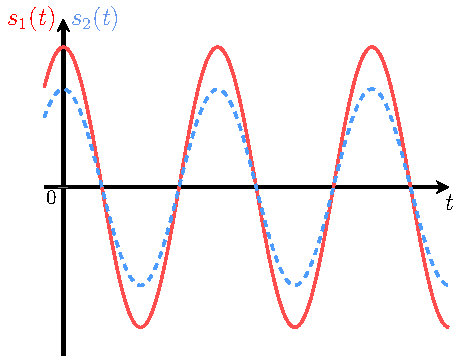
\includegraphics[width=\linewidth]{dfeq0.pdf}
		\captionof{figure}{En phase.}
	\end{center}
\end{tcb}

\begin{tcb}[sidebyside, righthand ratio=.25](defi)<lft>{Quadrature de phase}
	Deux signaux sont en \textbf{quadrature phase} si leur déphasage est de
	$\mathbf{\pm\pi/2}$ (modulo $2\pi$)~:
	\[
		\D\f \equiv \pm\frac{\pi}{2} \quad[2\pi]
		\Lra
		\boxed{\D\f = \left( p+\frac{1}{2} \right)\pi}
	\]
	Quand un signal s'annule, l'autre est à son maximum où à son minimum~:
	c'est la relation entre un cosinus et un sinus.
	\tcblower
	\begin{center}
		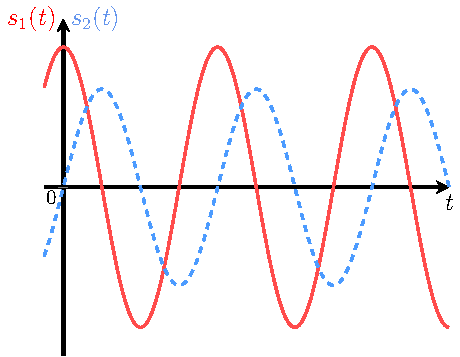
\includegraphics[width=\linewidth]{dfeqpi2.pdf}
		\captionof{figure}{Quadrature.}
	\end{center}
\end{tcb}

\begin{tcb}[sidebyside, righthand ratio=.25](defi)<lft>{Opposition de phase}
	Deux signaux sont en \textbf{opposition de phase} si leur déphasage est de
	$\mathbf{\pm\pi}$ (modulo $2\pi$)~:
	\[
		\D\f \equiv \pm\pi \quad[2\pi]
		\Lra
		\boxed{\D\f = (2p+1)\pi}
	\]
	Lorsqu'un signal passe par sa valeur maximale, l'autre est à la valeur
	minimale, mais ils s'annulent simultanément.
	\tcblower
	\begin{center}
		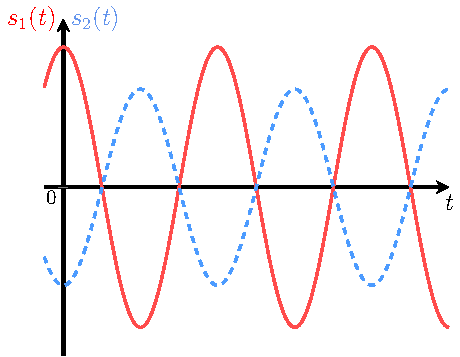
\includegraphics[width=\linewidth]{dfeqpi.pdf}
		\captionof{figure}{Opposition.}
	\end{center}
\end{tcb}

\subsection{Lecture d'un déphasage}
Le déphasage $\D\f_{2/1} = \f_2 - \f_1$ est lié au \textbf{retard temporel}
$\tau_{1/2}$ du signal $s_1$ par rapport au signal $s_2$~: on a
\[\boxed{\D\f_{2/1} = -\w\tau_{2/1}}\]

\begin{minipage}{0.70\linewidth}
	Dans ce cas, le déphasage obtenu est entre $-\pi$ et $+\pi$. On définit alors~:
	\begin{itemize}
		\item $\D\f_{2/1} > 0 \Rightarrow s_2$ est en avance sur $s_1$~;
		\item $\D\f_{2/1} < 0 \Rightarrow s_2$ est en retard sur $s_1$.
	\end{itemize}
\end{minipage}
\begin{minipage}{0.30\linewidth}
	\begin{center}
		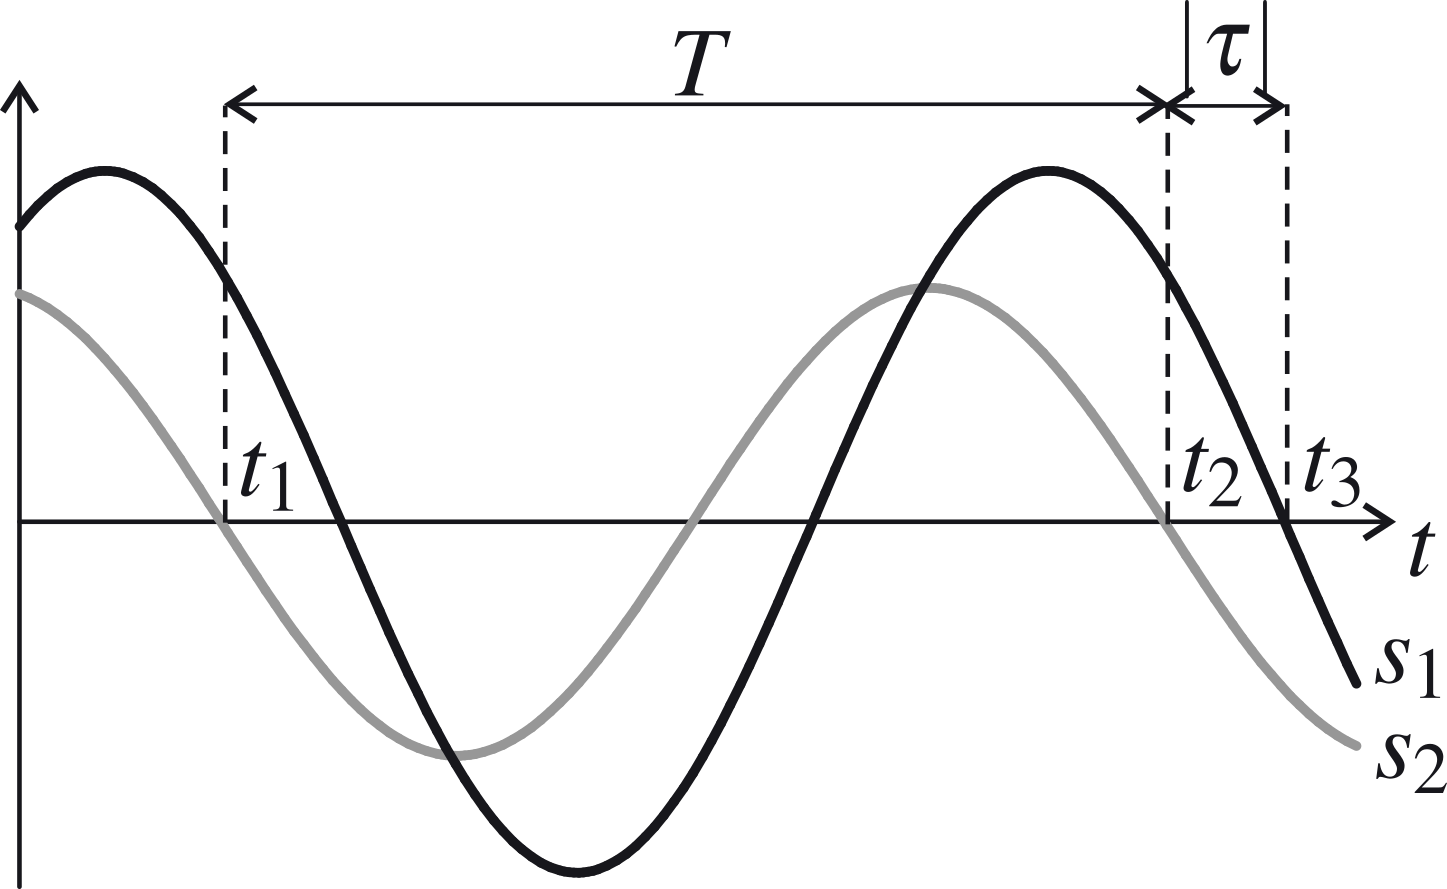
\includegraphics[width=\linewidth]{dfretard}
	\end{center}
\end{minipage}

Le principe est de mesurer la différence de temps entre les deux moments les
plus proches tels que les deux signaux s'annulent \textbf{avec la même pente}.
Par construction, la pulsation représente une vitesse angulaire, c'est pourquoi
on a $\w = 2\pi/T$ comme $v = d/t$ en mécanique. On trouve donc naturellement la
relation entre $\D\f_{2/1}$ et $\tau_{2/1}$.

\section{Superposition d'ondes sinuso\"idales de mêmes fréquences}
\subsection{Introduction}

La plupart du temps, les ondes se croisent sans interagir particulièrement, et
on ne voit que la somme des signaux. Voir l'animation
\texttt{geogebra}\footnote{\url{https://www.geogebra.org/m/jyh2ZMXJ}}. Étudions
mathématiquement ce phénomène en utilisant \textbf{deux sources sinusoïdales}.

\begin{tcb}(defi)<lft>'l'{Hypothèses}
	\begin{itemize}
		\item Chaque source émet un signal sinusoïdal~;
		\item Les deux signaux ont la même fréquence.
	\end{itemize}
\end{tcb}
\noindent
On pose donc
\[
	s_1(t) = A_1\cos(\wt+\f_1(\Mr))
	\qet
	s_2(t) = A_2\cos(\wt+\f_2(\Mr))
\]
les signaux en un point M de l'espace avec $\f_i(\Mr)$ le \textbf{déphasage
	spatial} du signal $i$. On s'intéresse au signal
\[s(t) = s_1(t) + s_2(t)\]

\subsection{Signaux de même amplitude}
\subsubsection{Cas général}

\leftcenters{\indent Commençons par étudier le cas où}{$\boxed{A_1 = A_2 = A_0}$}

On a alors
\begin{tcb}(exem)<lft>'l'{\small Développement}
	\vspace{-24pt}\psw{
		\begin{align*}
			s(t) & = s_1(t) + s_2(t)                                              \\
			     & = A_0 \left[ \cos(\wt+\f_1(\Mr)) + \cos(\wt+\f_2(\Mr)) \right] \\
			     & = 2A_0
			\cos \left( \frac{\wt + \f_1(\Mr) + \wt + \f_2(\Mr)}{2} \right)
			\cos \left( \frac{\wt + \f_1(\Mr) - \wt - \f_2(\Mr)}{2} \right)
		\end{align*}}
	\vspace{-24pt}
\end{tcb}

\begin{tcb}(rapp)<lfnt>'l'{Rappel}
	\vspace{-10pt}
	On a utilisé ici la formule
	\[\cos p + \cos q =
		2\cos \left( \frac{p+q}{2} \right)\cos \left( \frac{p-q}{2} \right)\]
	\vspace{-24pt}
\end{tcb}

Pour plus de lisibilité, on introduit donc
\[
	\D\f_{1/2}(\Mr) = \f_1(\Mr) - \f_2(\Mr)
	\qet
	\f_0(\Mr) = \frac{\f_1(\Mr)+\f_2(\Mr)}{2}
\]
\begin{tcb}(prop){Résultat}
	\psw{
		\leftcenters{Ainsi,}
		{$\DS s(t) = 2A_0\cos \left( \frac{\D\f_{1/2}(\Mr)}{2}
				\right)\cos(\wt+\f_0(\Mr))$}}
	\vspace{-15pt}
\end{tcb}
\begin{tcb}(ror){Analyse}
	Le signal somme de deux signaux sinusoïdaux de même amplitude $A_0$ et de
	même pulsation $\w$ est~:
	\begin{enumerate}
		\item Un signal \textbf{sinusoïdal} et \textbf{de même pulsation
			      $\mathbf{\w}$}~;
		\item D'amplitude \textbf{dépendante de $\mathbf{\D\f_{1/2}(\Mr)}$}, telle que
		      $A = 2A_0\cos\dfrac{\D\f_{1/2}(\Mr)}{2}$.
	\end{enumerate}

	\begin{minipage}{0.45\linewidth}
		\begin{center}
			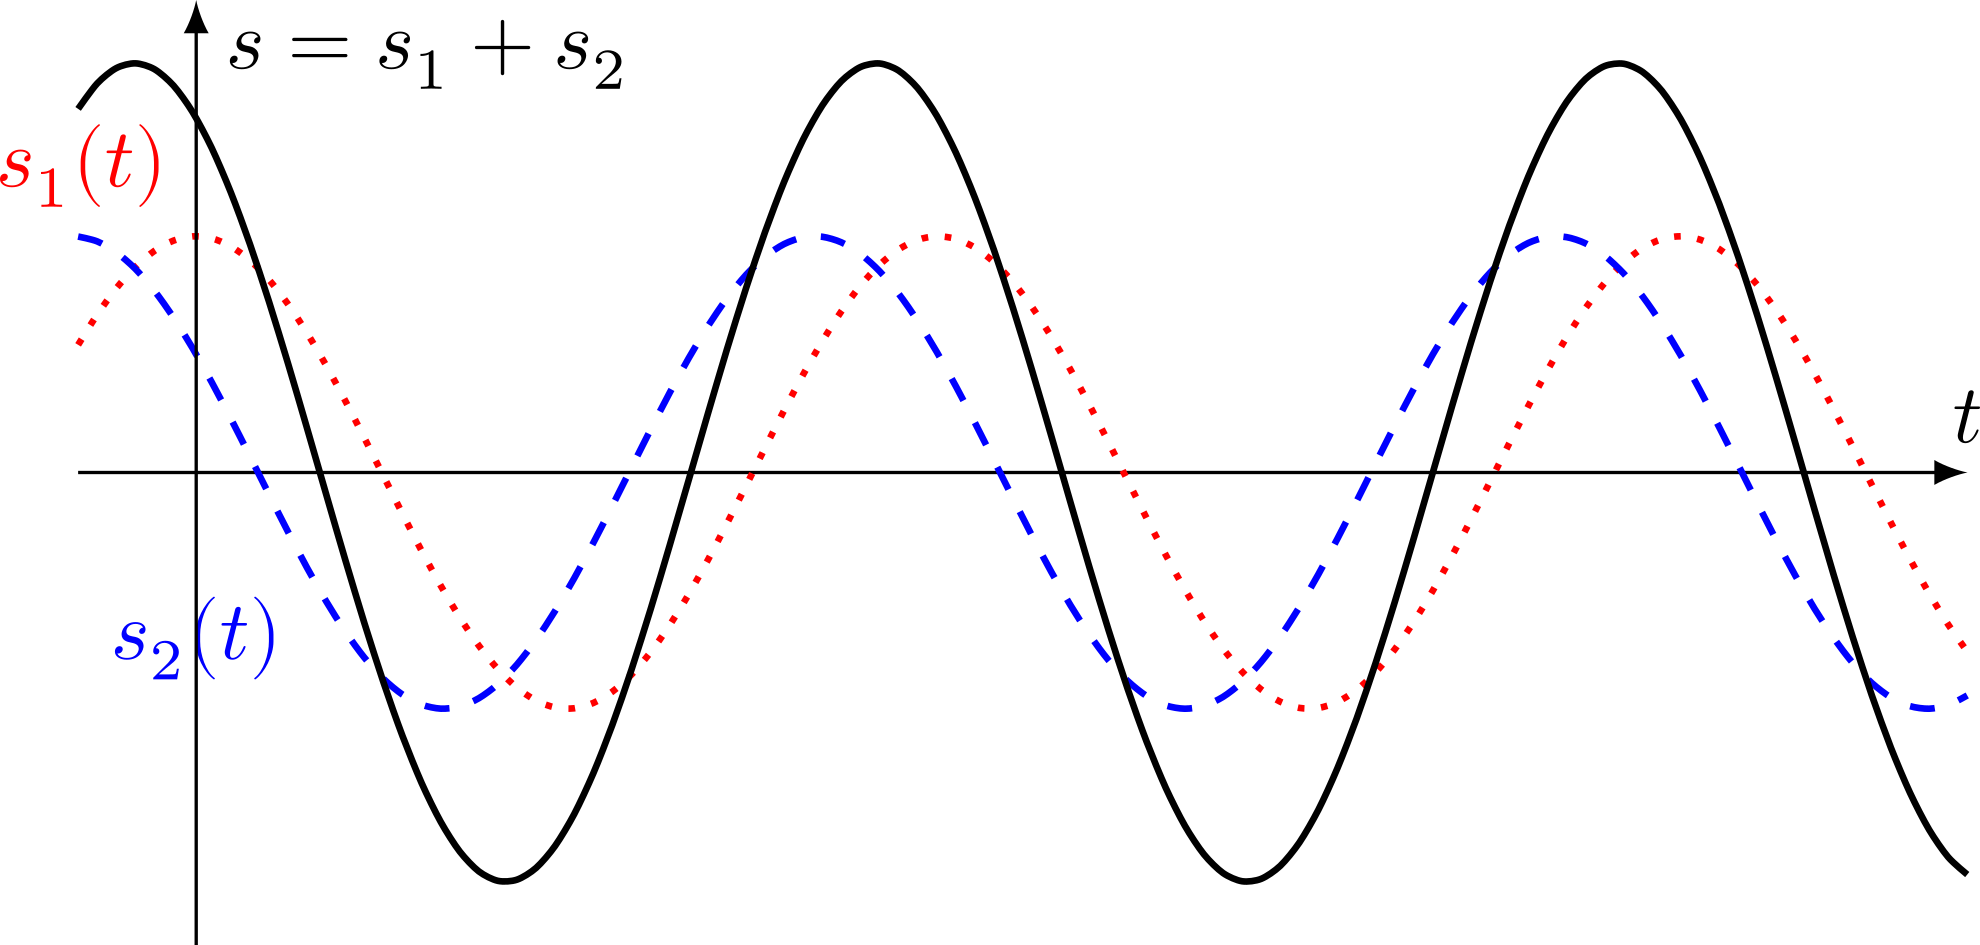
\includegraphics[width=\linewidth]{somme_pi3}
			\captionof{figure}{Somme avec déphasage $\D\f_{1/2} = \pi/3$.}
			\label{fig:sommepi3}
		\end{center}
	\end{minipage}
	\hfill
	\begin{minipage}{0.45\linewidth}
		\begin{center}
			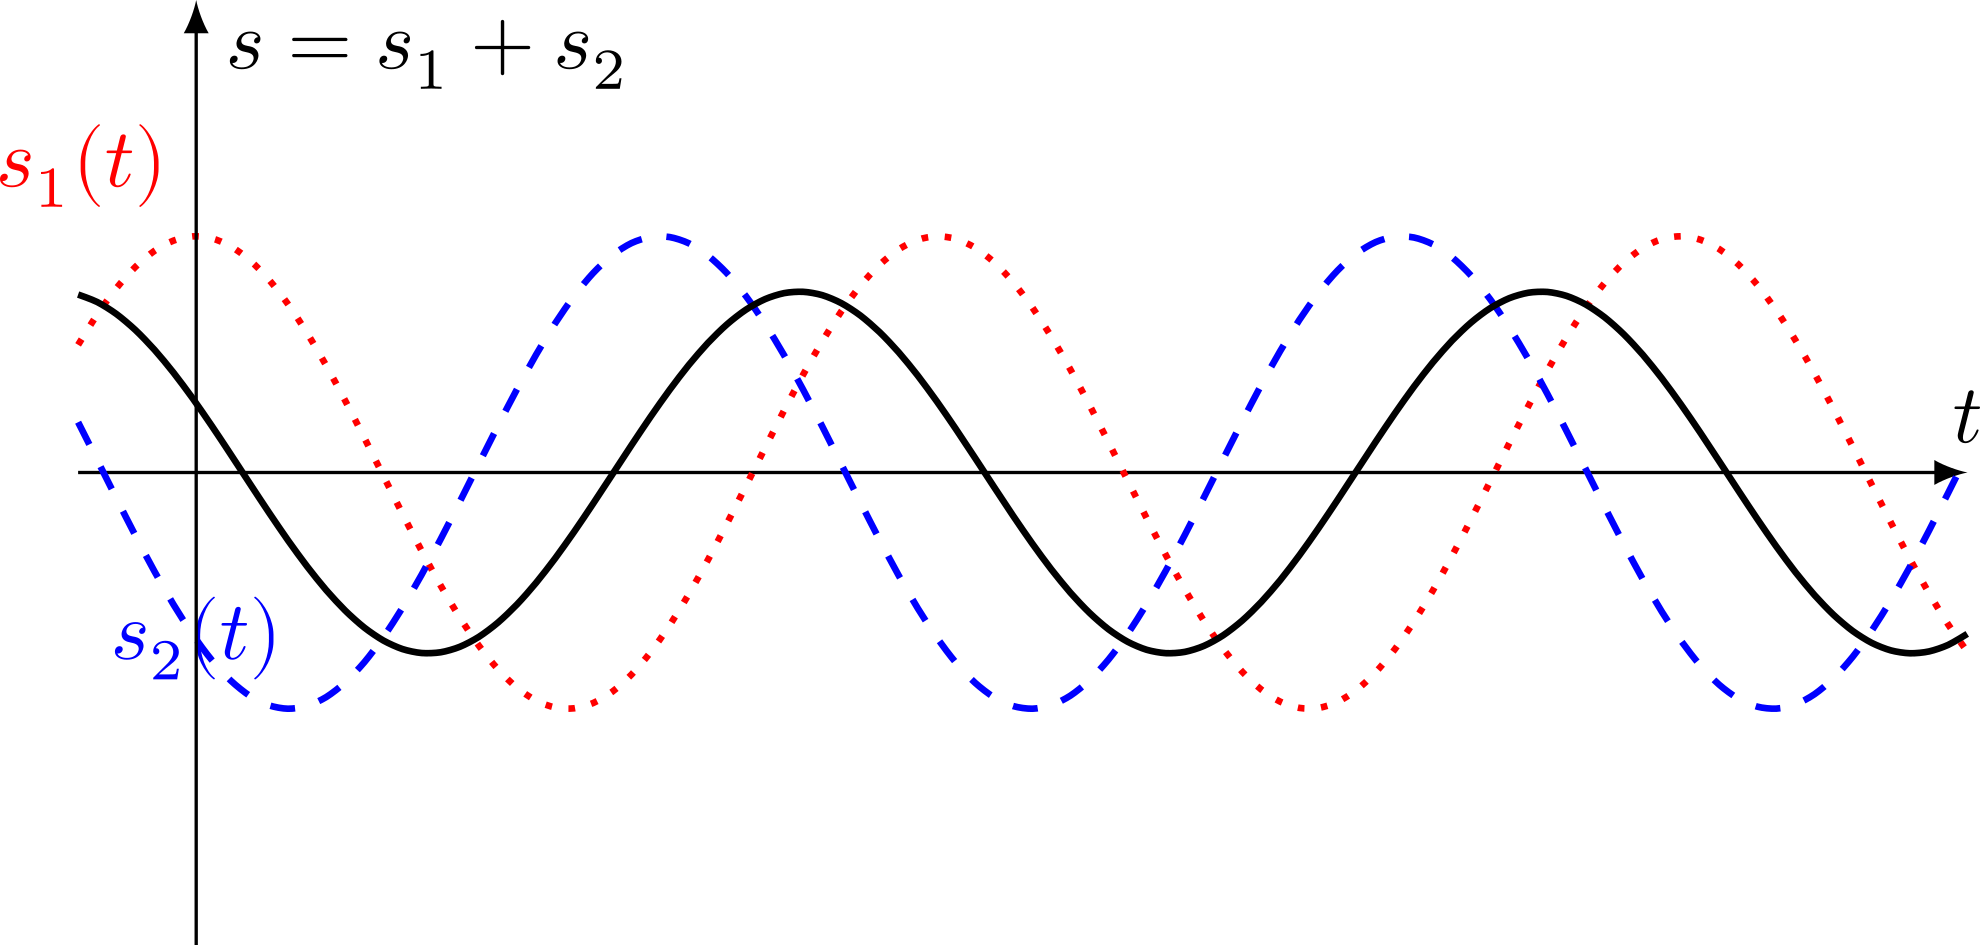
\includegraphics[width=\linewidth]{somme_3pi4}
			\captionof{figure}{Somme avec déphasage $\D\f_{1/2} = 3\pi/4$.}
			\label{fig:somme3pi4}
		\end{center}
	\end{minipage}
\end{tcb}

\vspace{-10pt}
\subsubsection{Cas extrêmes}
On distingue deux cas particuliers extrêmes avec cette formule~:

\begin{enumerate}[label=$\triangleright$]
	\item $\DS \cos \left( \frac{\D\f_{1/2}(\Mr)}{2} \right) = \pm 1$~: dans ce cas
	      \textbf{l'amplitude est maximale} et vaut $2A_0$. Or,
	      \[\psw{
			      \cos \left( \frac{\D\f_{1/2}(\Mr)}{2} \right) = \pm 1
			      \quad\Longleftrightarrow\quad
			      \frac{\D\f_{1/2}(\Mr)}{2} p\pi
			      \quad\Longleftrightarrow\quad
			      \D\f_{1/2}(\Mr) = 2p\pi
		      }\]
	      Ce déphasage correspond à des \textbf{signaux en phase}. Ainsi, lorsque
	      les signaux sont en phase, les maxima et minima de vibration se
	      correspondent pour donner à chaque instant une amplitude double.
	\item $\DS \cos \left( \frac{\D\f_{1/2}(\Mr)}{2} \right) = 0$~: dans ce cas,
	      \textbf{l'amplitude est nulle}. Or,
	      \[\psw{
			      \cos \left( \frac{\D\f_{1/2}(\Mr)}{2} \right) = 0
			      \quad\Longleftrightarrow\quad
			      \frac{\D\f_{1/2}(\Mr)}{2} = p\pi + \frac{\pi}{2}
			      \quad\Longleftrightarrow\quad
			      \D\f_{1/2}(\Mr) = (2p+1)\pi
		      }\]
	      Ce sont donc des \textbf{signaux en opposition de phase}. Ainsi, des
	      signaux en opposition de phase ont leurs minima et maxima qui
	      s'opposent, et l'amplitude résultante est nulle.
\end{enumerate}
Ceci est vérifiable avec l'animation \texttt{geogebra}.


\subsection{Signaux d'amplitudes différentes}
\subsubsection{Cas général}
\leftcentersright{On a toujours}{$s(t) = s_1(t) + s_2(t)$}{mais $A_1\neq A_2$.}

\noindent
On note simplement $\f_1$ et $\f_2$ dans les calculs pour alléger l'écriture.
On peut soit utiliser la trigonométrie classique, soit les complexes~:
\begin{tcb}[sidebyside](rapp){Rappel}
	\vspace*{-15pt}
	\begin{align*}
		\cos(a+b) & = \cos a\cos b - \sin a\sin b \\
		\cos(a-b) & = \cos a\cos b + \sin a\sin b
	\end{align*}
	\tcblower
	\vspace*{-15pt}
	\begin{gather*}
		\cos\theta = \frac{\exr^{\jj\theta}+\exr^{-\jj\theta}}{2}\\
		\abs{\zu}^2 = \zu\times\zu^*
		\qet
		\tan\arg*{\zu} = \frac{\Im(\zu)}{\Re(\zu)}
	\end{gather*}
\end{tcb}
Ce qui donne~:

\begin{tcb}[breakable](demo){Démonstration}
	\tcbsubtitle{\fatbox{En réels}}
	\vspace{-20pt}\psw{
		\begin{align*}
			s(t) & = A_1\cos(\wt+\f_1) + A_2\cos(\wt+\f_2)  \\
			\Leftrightarrow s(t)
			     & = A_1(\cos\wt\cos\f_1 - \sin\wt\sin\f_1) \\
			     & + A_2(\cos\wt\cos\f_2 - \sin\wt\sin\f_2) \\
			\Leftrightarrow s(t)
			     & = (A_1\cos\f_1+A_2\cos\f_2)\cos\wt       \\
			     & - (A_1\sin\f_1+A_2\sin\f_2)\sin\wt
		\end{align*}
		Ceci est équivalent à écrire
		\begin{gather*}
			\boxed{s(t) = A\cos(\wt+\f)}\qcar\\
			A\cos(\wt+\f) = A\cos\f\cos\wt - A\sin\f\sin\wt
		\end{gather*}
		On trouve donc
		\[
			\left\{
			\begin{array}{rcl}
				A\cos\f & = & A_1\cos\f_1 + A_2\cos\f_2\quad(1) \\
				A\sin\f & = & A_1\sin\f_1 + A_2\sin\f_2\quad(2)
			\end{array}
			\right.
		\]
		On obtient $A$ l'amplitude de l'onde somme en prenant $(1)^2+(2)^2$, et
		$\tan\f$ avec $(2)/(1)$~:
		\begin{gather*}
			\left\{
			\begin{array}{rcl}
				A^2\underbrace{(\cos^2\f + \sin^2\f)}_{=1}
				 & = &
				A_1{}^2 + A_2{}^2 + 2A_1A_2
				\underbrace{(\cos\f_1\cos\f_2 +
				\sin\f_1\sin\f_2)}_{=\cos(\f_1-\f_2)} \\[2em]
				\tan\f
				 & = &
				\dfrac{A_1\sin\f_1+A_2\sin\f_2}{A_1\cos\f_1+A_2\cos\f_2}
			\end{array}
			\right.\\[1em]
			\Leftrightarrow
			\left\{
			\begin{array}{rcl}
				A  & = & \sqrt{A_1{}^2+A_2{}^2 + 2A_1A_2\cos(\D\f_{1/2})} \\
				\f & = & \atan
				\left(
				\dfrac{A_1\sin\f_1+A_2\sin\f_2}{A_1\cos\f_1+A_2\cos\f_2}
				\right)
			\end{array}
			\right.
		\end{gather*}
	}\vspace{-10pt}
	\tcblower
	\tcbsubtitle{\fatbox{En complexes}}
	En supposant directement que $s(t) = A\cos(\wt+\f)$ (par linéarité),
	\psw{
		\begin{gather*}
			\begin{aligned}
				\xul{s}                             & = \xul{s_1} + \xul{s_2} \\
				\Leftrightarrow
				A\exr^{\jj\f}\cancel{\exr^{\jj\wt}} & =
				A_1\exr^{\jj\f_1}\cancel{\exr^{\jj\wt}} +
				A_2\exr^{\jj\f_2}\cancel{\exr^{\jj\wt}}                       \\
				\Leftrightarrow
				A\exr^{\jj\f}                       & =
				A_1\exr^{\jj\f_1} +
				A_2\exr^{\jj\f_2}
			\end{aligned}\\
			\begin{aligned}
				\text{D'où}\quad &
				\left\{
				\begin{array}{rcl}
					\abs{\xul{A}}^2 & = &
					(\xul{A_1}+\xul{A_2})(\xul{A_1}^* + \xul{A_2}^*) \\
					\arg*{\xul{A}}  & = & \arg*{\xul{A_1}+\xul{A_2}}
				\end{array}
				\right.            \\
				\Leftrightarrow  &
				\left\{
				\begin{array}{rcl}
					A^2 & = &
					(A_1\exr^{\jj\f_1}+A_2\exr^{\jj\f_2})  \times
					(A_1\exr^{-\jj\f_1}+A_2\exr^{-\jj\f_2})      \\
					\f  & = & \arg*{A_1\cos\f_1+ \jj A_1\sin\f_1
					+ A_2\cos\f_2 + \jj A_2\sin\f_2)}            \\
				\end{array}
				\right.            \\
				\Leftrightarrow  &
				\left\{
				\begin{array}{rcl}
					A^2    & = & A_1{}^2
					\underbrace{\exr^{\jj(\f_1-\f_1)}}_{=1} +
					A_2{}^2
					\underbrace{\exr^{\jj(\f_2-\f_2)}}_{=1} +
					+ A_1A_2
					\underbrace{\left(
						\exr^{\jj(\f_1-\f_2)} + \exr^{-\jj(\f_1-\f_2)}
					\right)}_{=2\cos\D\f_{1/2}} \\[2em]
					\tan\f & = &
					\dfrac{A_1\sin\f_1+A_2\sin\f_2}
					{A_1\cos\f_1+A_2\cos\f_2}
				\end{array}
				\right.            \\
				\Leftrightarrow  &
				\left\{
				\begin{array}{rcl}
					A  & = & \sqrt{A_1{}^2+A_2{}^2 + 2A_1A_2\cos(\D\f_{1/2})} \\
					\f & = & \atan
					\left(
					\dfrac{A_1\sin\f_1+A_2\sin\f_2}{A_1\cos\f_1+A_2\cos\f_2}
					\right)
				\end{array}
				\right.
			\end{aligned}
		\end{gather*}}
	\hspace{-20pt}
	\hdashrule[0.5ex]{1.05\linewidth}{.5pt}{3pt}
	Dans tous les cas, on appelle donc
	\[\f_0(\Mr) =
		\atan
		\left(
		\dfrac{A_1\sin\f_1+A_2\sin\f_2}{A_1\cos\f_1+A_2\cos\f_2}
		\right)
	\]
	et ainsi,
\end{tcb}
\begin{tcb}(prop){Résultat}
	\[\psw{
		s(t) = \sqrt{A_1{}^2+A_2{}^2 + 2A_1A_2\cos(\D\f_{1/2}(\Mr))}\cos(\wt+\f_0(\Mr))
		}\]
\end{tcb}

Ainsi, même si les amplitudes sont différentes le résultat fondamental reste le
même~: l'amplitude dépend du déphasage et il y a possibilité d'avoir des
interférences constructives et destructives. Les minima et maxima ne sont
cependant \textbf{plus les mêmes}.

\subsubsection{Cas extrêmes}

\begin{enumerate}[label=$\triangleright$]
	\item $\DS \cos \D\f_{1/2} = 1$~: dans ce cas
	      \textbf{l'amplitude est maximale} et vaut
	      $\sqrt{A_1{}^2+A_2{}^2+2A_1A_2} = A_1+A_2$. Or,
	      \[\psw{
			      \cos \D\f_{1/2} = 1
			      \quad\Longleftrightarrow\quad
			      \D\f_{1/2} = 2p\pi
		      }\]
	      Ce déphasage correspond à des \textbf{signaux en phase}. Ainsi, lorsque
	      les signaux sont en phase, les maxima et minima de vibration se
	      correspondent pour donner à chaque instant une amplitude égale à la
	      somme des deux.
	\item $\DS \cos \D\f_{1/2} = -1$~: dans ce cas \textbf{l'amplitude est minimale}
	      et vaut $\sqrt{A_1{}^2+A_2{}^2-2A_1A_2} = \abs{A_1-A_2}$. Or,
	      \[\psw{
			      \cos \D\f_{1/2} = -1
			      \quad\Longleftrightarrow\quad
			      \D\f_{1/2} (2p+1)\pi
		      }\]
	      Ce sont donc des \textbf{signaux en opposition de phase}. Ainsi, des
	      signaux en opposition de phase ont leurs minima et maxima qui
	      s'opposent, et l'amplitude résultante est minimale.
\end{enumerate}
\begin{tcb}(ror){Analyse}
	Le signal somme de deux signaux sinusoïdaux d'amplitudes $A_1$ et $A_2$ de
	même pulsation $\w$ est~:
	\begin{enumerate}
		\item Un signal \textbf{sinusoïdal} et \textbf{de même pulsation
			      $\mathbf{\w}$}~;
		\item D'amplitude \textbf{dépendante de $\mathbf{\D\f_{1/2}(\Mr)}$}, telle que
		      \[\boxed{A = \sqrt{A_1{}^2+A_2{}^2 + 2A_1A_2\cos(\D\f_{1/2}(\Mr))}}\]
		      \begin{itemize}
			      \item \textbf{Maximale} $A_1 + A_2$ pour signaux \textbf{en
				            phase} ($\D\f_{1/2} = 2p\pi$, $p\in\Zb$)~;
			      \item \textbf{Minimale} $A_1 - A_2$ pour signaux \textbf{en
			            opposition de phase} ($\D\f_{1/2} = (2p+1)\pi$, $p\in\Zb$).
		      \end{itemize}
	\end{enumerate}
	\begin{minipage}{0.45\linewidth}
		\begin{center}
			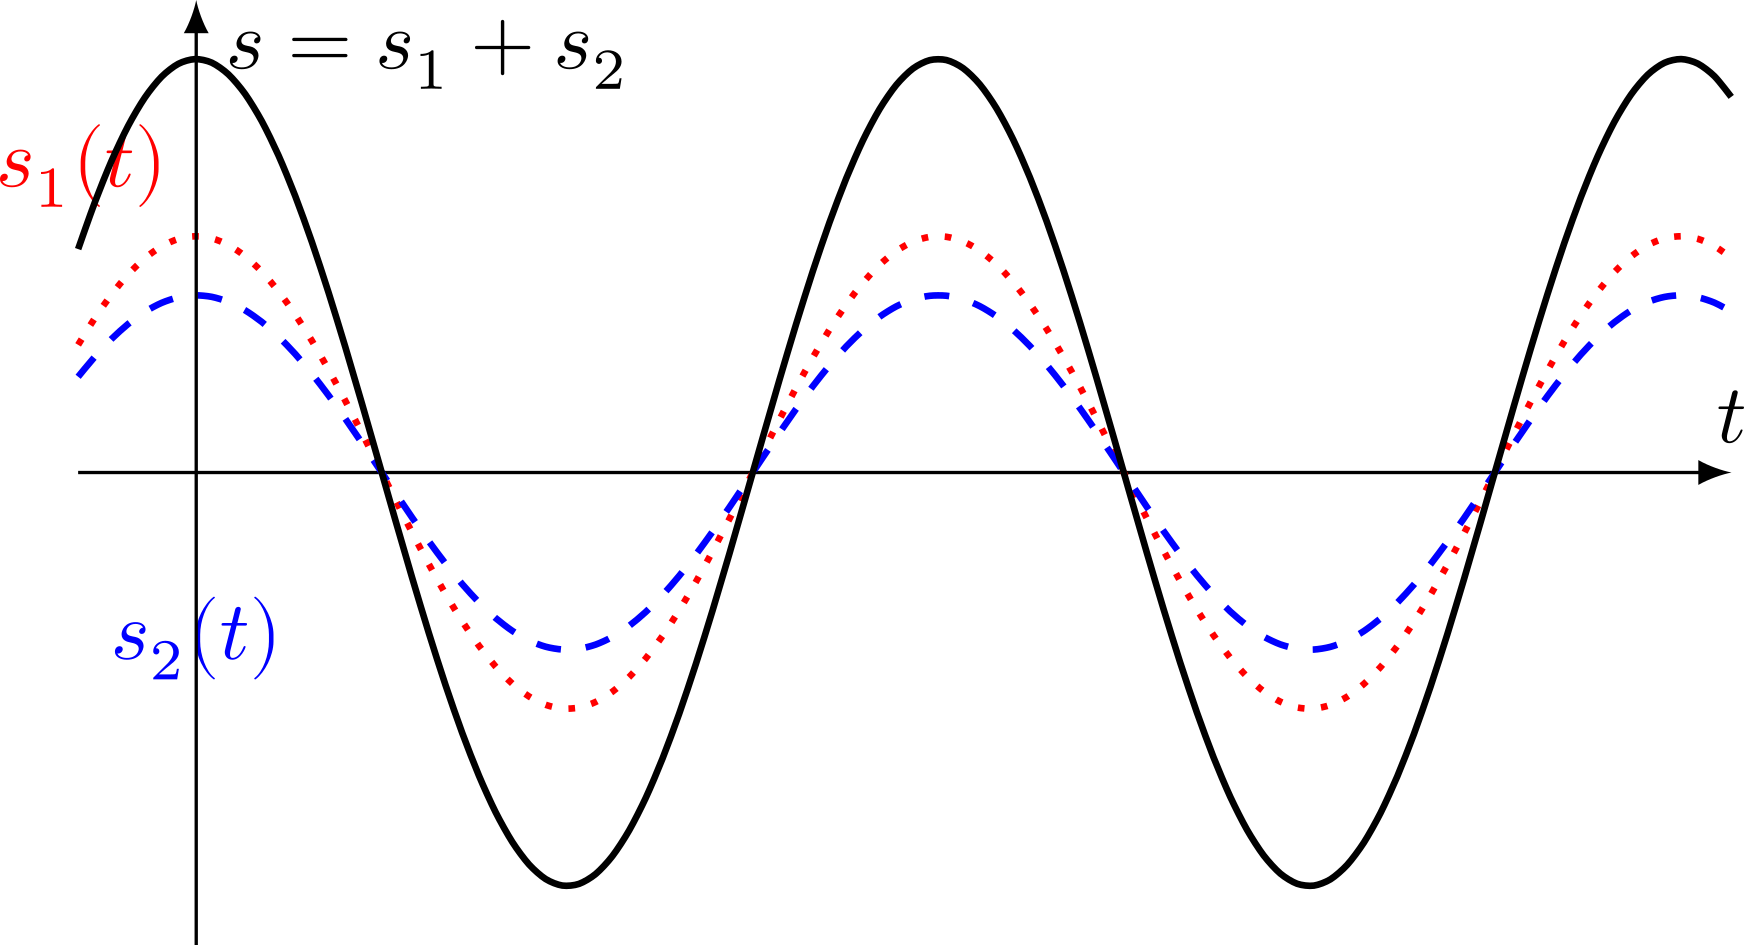
\includegraphics[width=\linewidth]{somme_0}
			\captionof{figure}{Signaux en phase.}
			\label{fig:sommephase}
		\end{center}
	\end{minipage}
	\hfill
	\begin{minipage}{0.45\linewidth}
		\begin{center}
			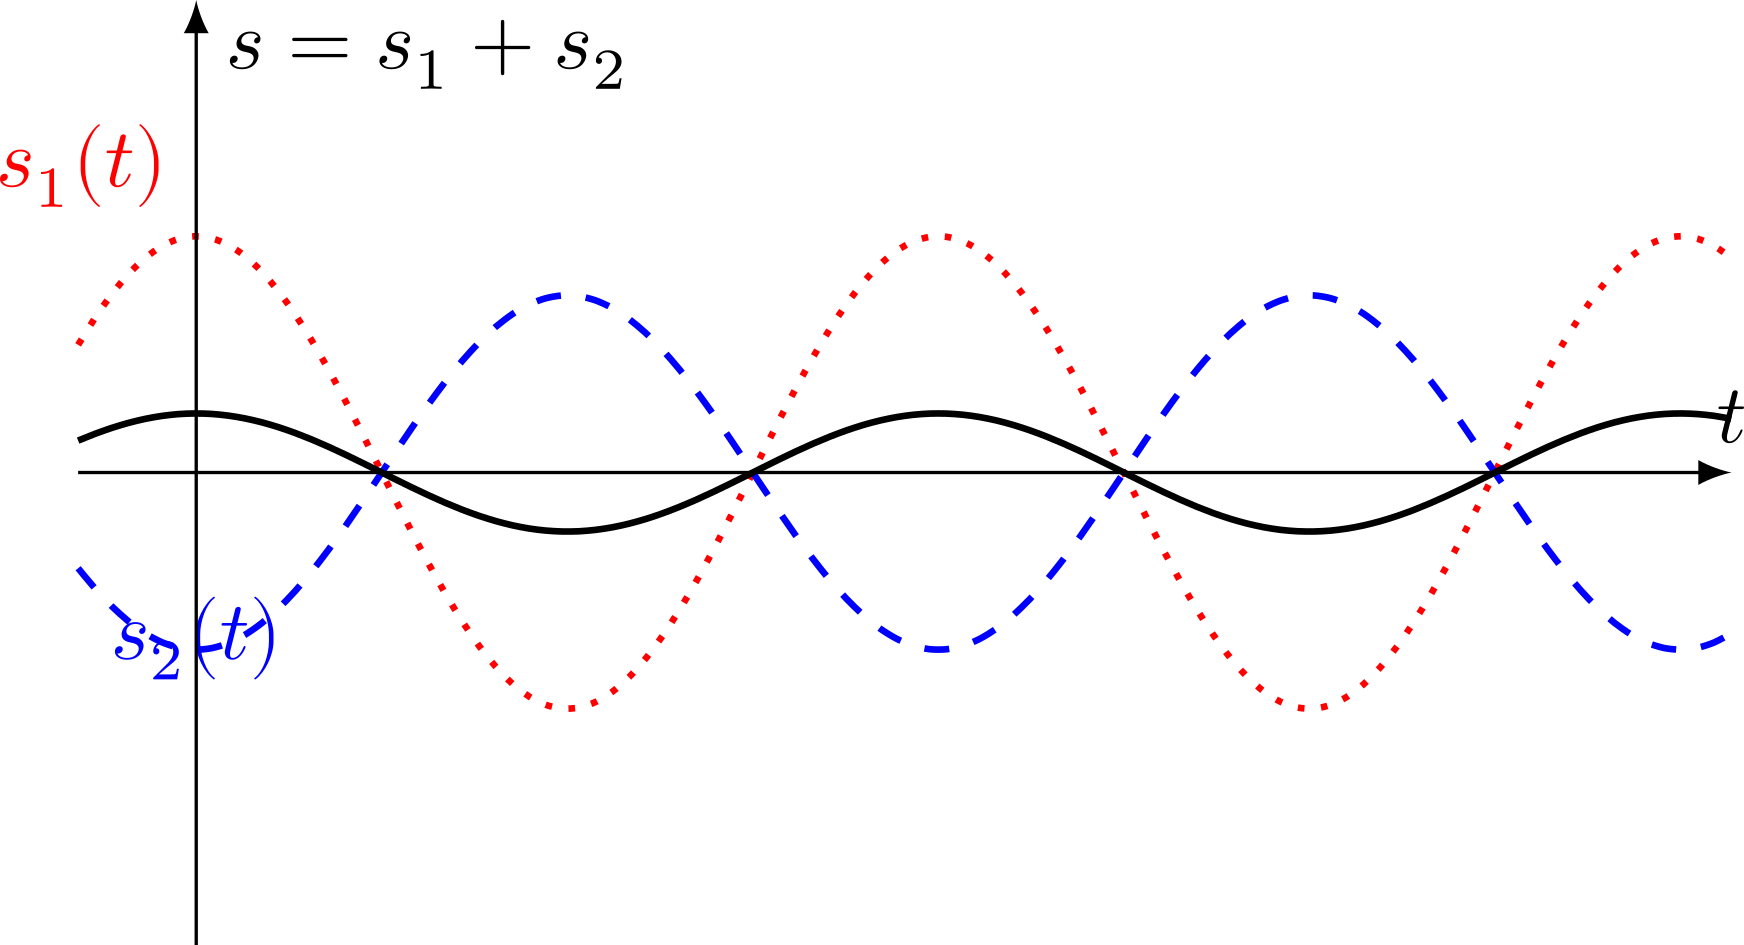
\includegraphics[width=\linewidth]{somme_pi}
			\captionof{figure}{Signaux en opposition.}
			\label{fig:sommeopp}
		\end{center}
	\end{minipage}
\end{tcb}

\subsection{Bilan}

\begin{tcb}[breakable](ror){Bilan}
	Lorsque deux ondes \textbf{de même fréquence} et de \textbf{même nature} se
	superposent en M~:
	\begin{isd}
		L'amplitude de la somme est \textbf{maximale} si les signaux sont
		\textbf{en phase}~:
		\[\boxed{\D\f_{1/2}(\Mr) = \f_2(\Mr)-\f_1(\Mr) = 2p\pi}\]
		On parle d'\textbf{interférences constructives}.
		\tcblower
		L'amplitude de la somme est \textbf{minimale} si les signaux sont
		\textbf{en opposition de phase}~:
		\[\boxed{\D\f_{1/2}(\Mr) = \f_2(\Mr)-\f_1(\Mr) = (2p+1)\pi}\]
		On parle d'\textbf{interférences destructives}.
	\end{isd}
	\centering$p\in\Zb$ est appelé l'\textbf{ordre d'interférence}.
\end{tcb}

\section{Approximation par une onde plane}
\subsection{Sources ponctuelles}
\begin{minipage}{0.55\linewidth}
	D'une manière générale, une source ponctuelle émet une onde dans tout l'espace
	disponible~:
	\begin{itemize}
		\item Si c'est une \textbf{droite}, alors l'onde est \textbf{plane}~;
		\item Si c'est un \textbf{plan}, alors l'onde est \textbf{circulaire}~;
		\item Si c'est un \textbf{volume}, alors l'onde est \textbf{sphérique}.
	\end{itemize}
\end{minipage}
\hfill
\begin{minipage}{0.35\linewidth}
	\begin{center}
		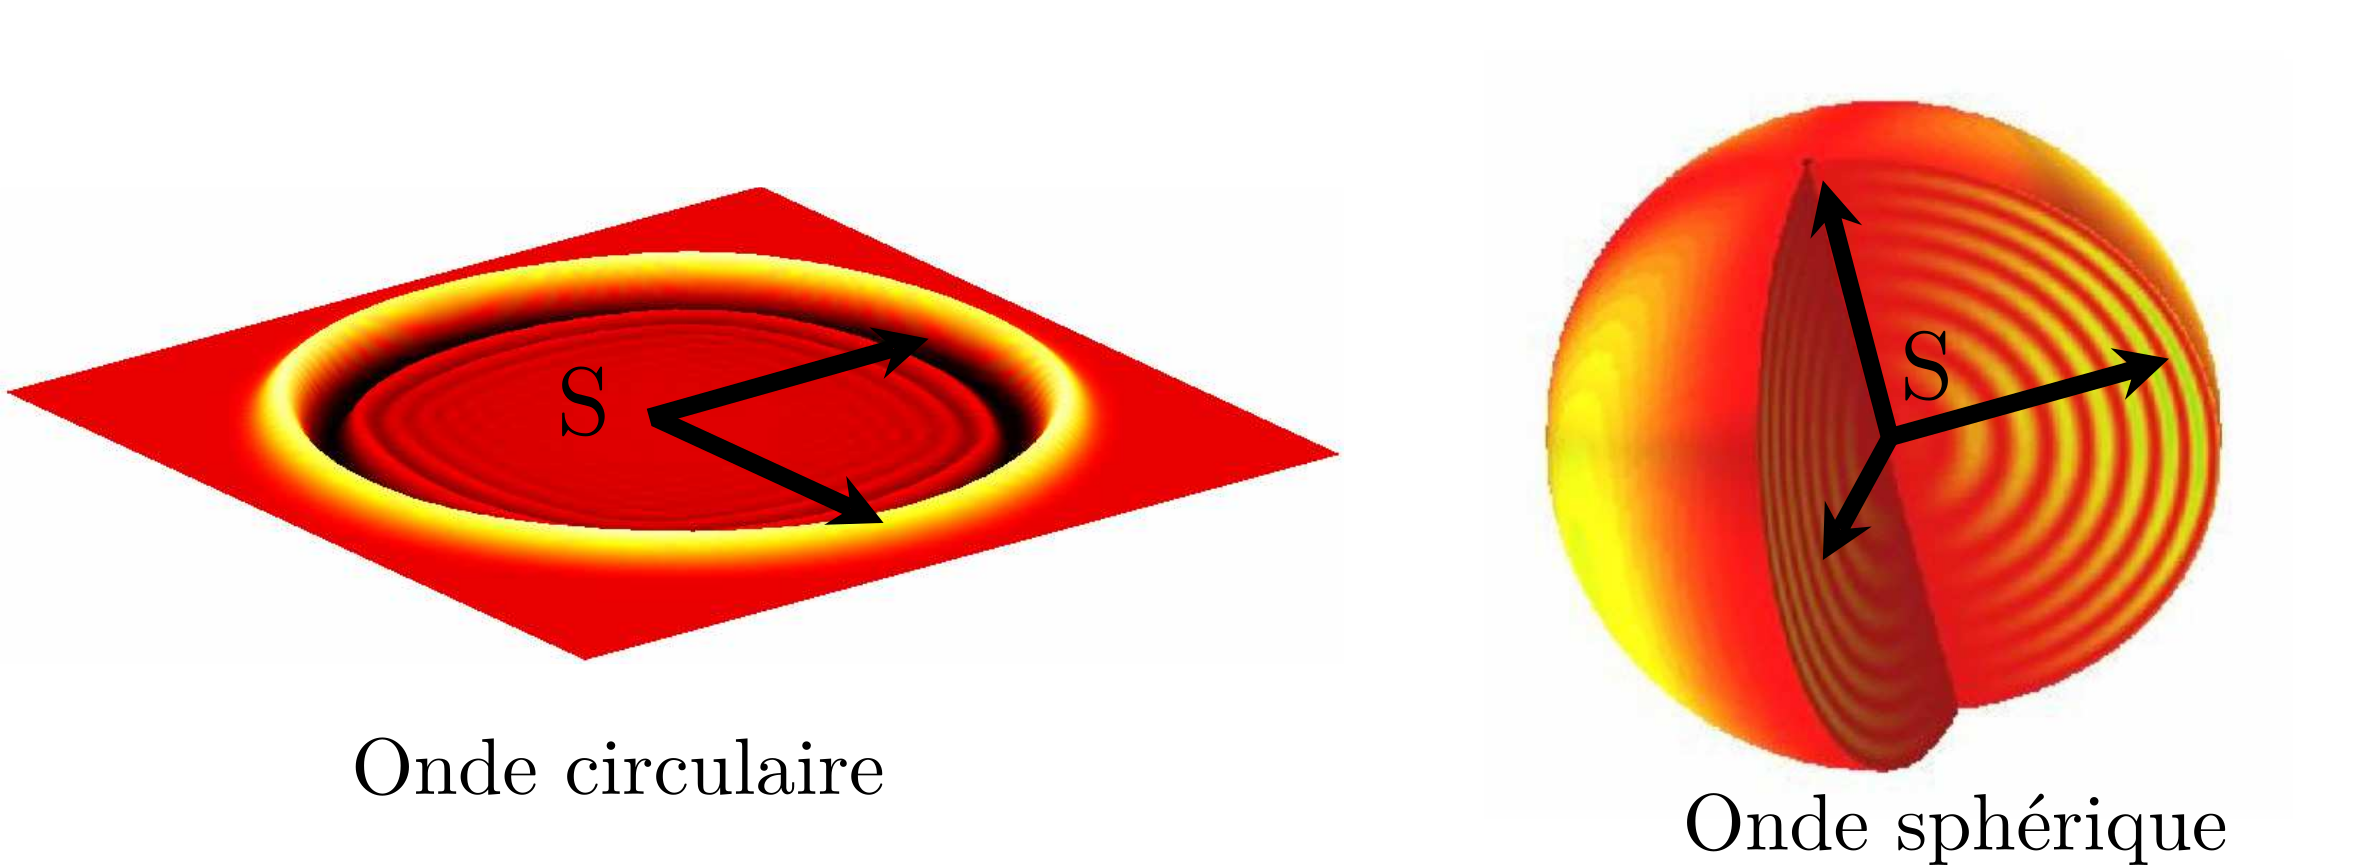
\includegraphics[width=\linewidth]{ondes_c_s}
	\end{center}
\end{minipage}\bigbreak

Pour que l'étude précédente fonctionne, il faut que les signaux soient de la
même forme mathématique. On utilise pour cela l'approximation suivante~:

\begin{tcb}[sidebyside, righthand ratio=.4](prop){Approximation par une onde plane}

	À des distances de la source suffisamment grandes devant la longueur
	d'onde $\lambda$, on peut approximer la vibration $s(\Mr,t)$ en un point
	M d'une onde circulaire ou sphérique par une onde place, telle que
	\psw{
		\[\boxed{s(\Mr,t) = A\cos(\wt-k\SMr +\f_S)}\]
	}
	avec $A$ constante au
	voisinage de M et $\f_S$ la phase à l'origine des temps de la source.
	\tcblower
	\begin{center}
		\sswitch{
			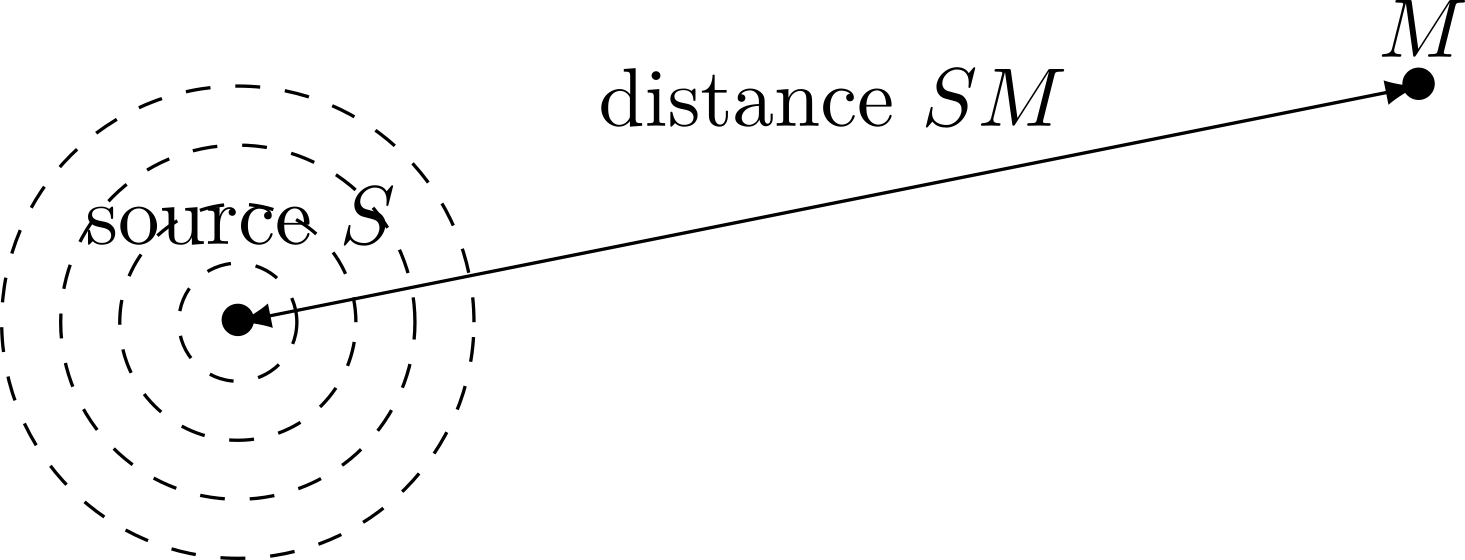
\includegraphics[width=\linewidth, draft=true]{SM}
		}{
			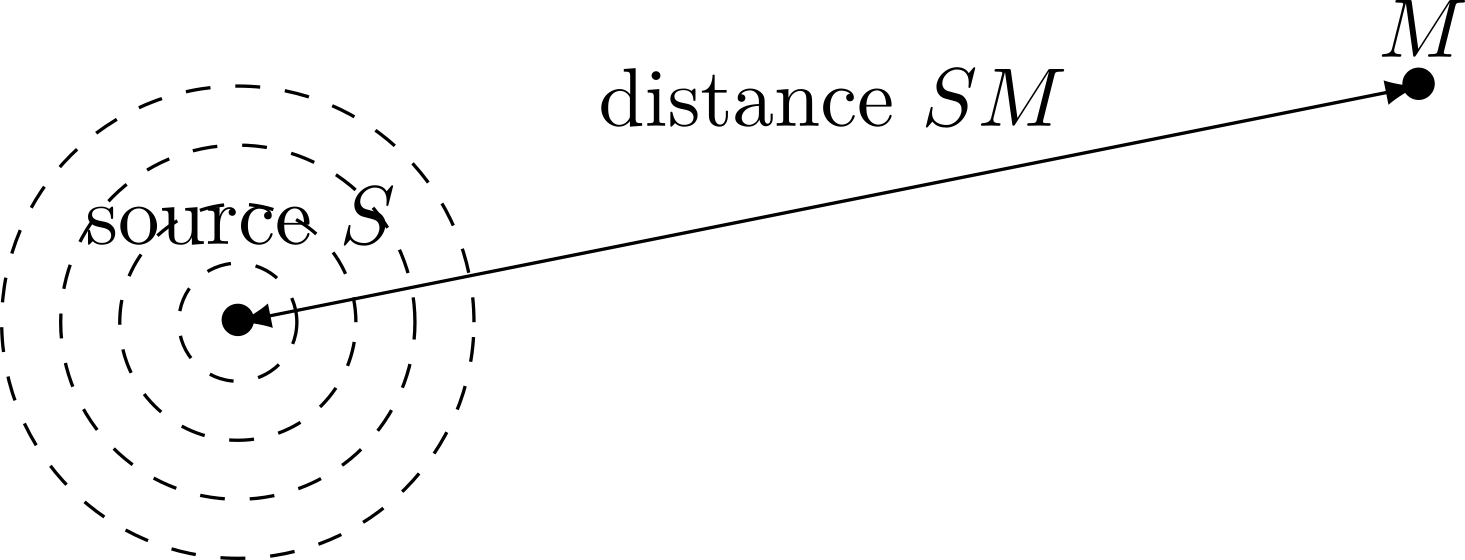
\includegraphics[width=\linewidth]{SM}
		}
		\captionof{figure}{Approximation par une onde plane}
	\end{center}
\end{tcb}

\subsection{Déphasage et différence de marche}
\noindent
\begin{minipage}{0.65\linewidth}
	Supposons deux sources S$_1$ et S$_2$ émettant chacune une onde sphérique
	sinusoïdale \textbf{à la même pulsation} et de \textbf{même longueur d'onde}.
	Suffisamment loin de la source, elles peuvent se mettre sous la forme~:
\end{minipage}
\hfill
\begin{minipage}{0.30\linewidth}
	\begin{center}
		\sswitch{
			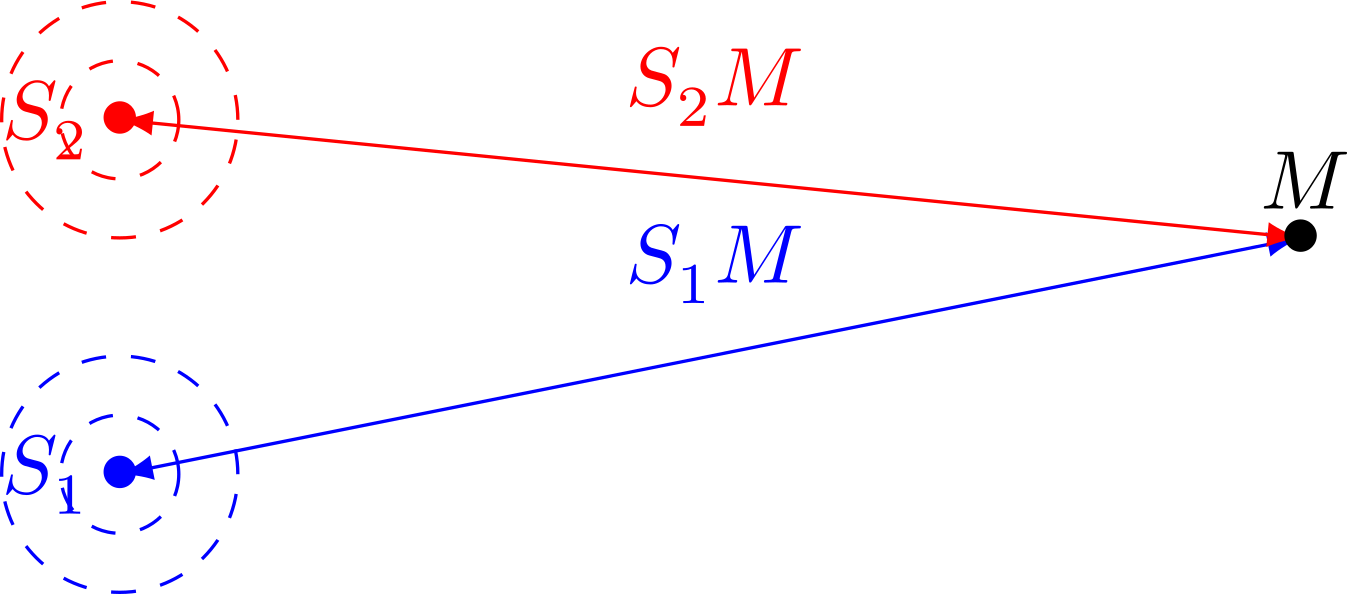
\includegraphics[width=\linewidth]{S12M}
		}{
			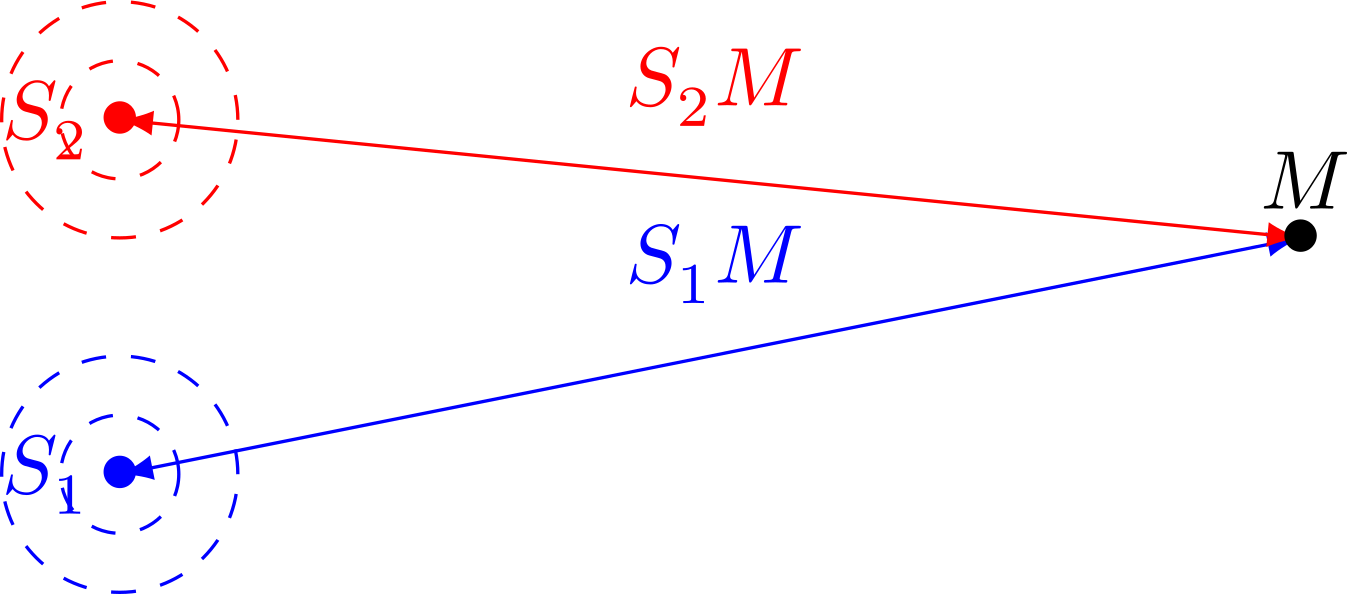
\includegraphics[width=\linewidth]{S12M}
		}
		\vspace{-15pt}
		\captionof{figure}{S$_1$ et S$_2$.}
	\end{center}
\end{minipage}
\psw{
	\[
		s_1(\Mr,t) = A_1\cos(\wt - k\SaMr + \f_{01})
		\qet
		s_2(\Mr,t) = A_2\cos(\wt - k\SbMr + \f_{02})
	\]
}
On aura donc
\psw{
	\[
		\f_1(\Mr) = -k\SaMr + \f_{01}
		\qet
		\f_2(\Mr) = -k\SaMr + \f_{02}
	\]
}
Le déphasage au point M est donc
\psw{
	\[\D\f_{1/2}(\Mr) = \f_1(\Mr) - \f_2(\Mr) = -k(\SaMr - \SbMr) + \f_{01} -
		\f_{02}\]
}

\begin{tcb}(prop){Déphasage et différence de marche}
	Le déphasage entre 2 ondes se superposant en M est
	\[\psw{
			\boxed{\D\f_{1/2}(\Mr) = -k\D L_{1/2}(\Mr) + \D\f_0}
			\qav k=\frac{2\pi}{\lambda}}\]
	\begin{itemize}
		\item $\D L_{1/2}(\Mr) = \SaMr - \SbMr$ est la \textbf{différence de
			      marche} au point M. C'est la distance supplémentaire que doit
		      parcourir l'onde 1 par rapport à l'onde 2 pour qu'elle atteigne M.
		\item $\D\f_0 = \f_{01}-\f_{02}$ est la \textbf{différence de phase à
			      l'origine entre les sources}. Si elles sont identiques, on aura
		      simplement $\D\f_0 = 0$.
	\end{itemize}
\end{tcb}

\begin{tcb}(impl){Implication~: interférences \textit{via} différence de marche}
	Pour des sources de même phase à l'origine, on a donc $\Delta\f_0 = 0$, d'où
	\smallbreak
	\begin{isd}[sidebyside align=top]
		\tcbsubtitle{\fatbox{En phase}}
		\vspace{-15pt}
		\psw{
			\begin{gather*}
				\Delta\f_{1/2}(\Mr) = 2p\pi
				\\\Lra
				\boxed{\Delta{L}_{2/1}(\Mr) = p\lambda}
			\end{gather*}
		}
		\vspace{-15pt}
		\tcblower
		\tcbsubtitle{\fatbox{En opposition}}
		\vspace{-15pt}
		\psw{
			\begin{gather*}
				\Delta\f_{1/2}(\Mr) = (2p+1)\pi
				\\\Lra
				\boxed{\Delta{L}_{2/1}(\Mr) = \left(p+\frac{1}{2}\right)\lambda}
			\end{gather*}
		}
		\vspace{-15pt}
	\end{isd}
\end{tcb}

\begin{tcb}[breakable](appl){Exercice}
	\begin{minipage}{0.55\linewidth}
		Soient 2 émetteurs sonores envoyant une onde progressive sinusoïdale de
		même fréquence, amplitude et phase à l'origine. Le premier est fixé à
		l'origine du repère, l'émetteur 2 est mobile et à une distance $d$ du
		premier, et un microphone est placé à une distance fixe $x_0$ de
		l'émetteur 1 et est aligné avec les deux émetteurs. On néglige
		l'influence de l'émetteur 2 sur l'émetteur 1 et toute atténuation.
	\end{minipage}
	\hfill
	\begin{minipage}{0.45\linewidth}
		\begin{center}
			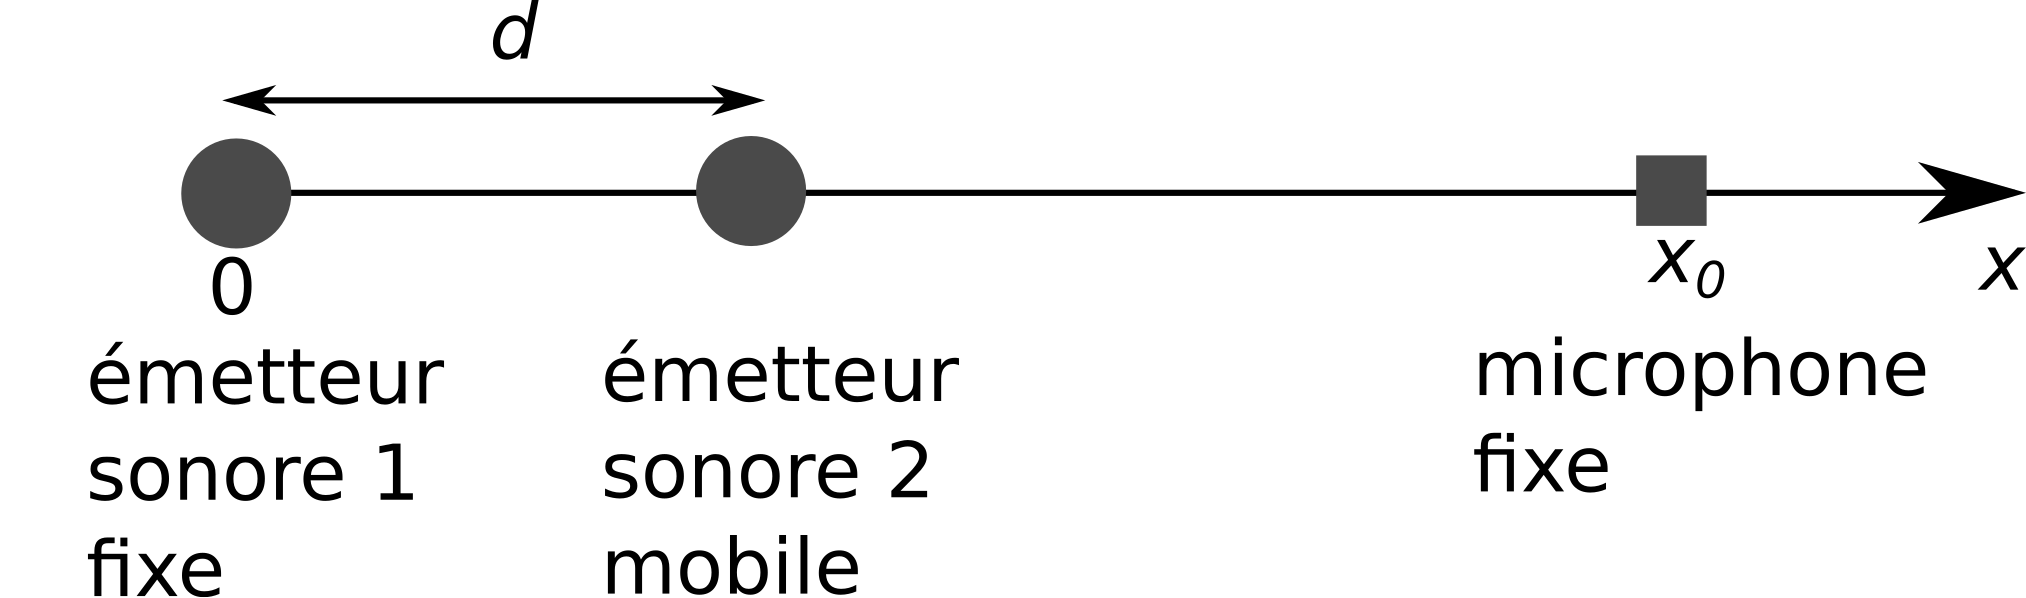
\includegraphics[width=\linewidth]{microphone}
		\end{center}
	\end{minipage}
	\begin{enumerate}[label=\sqenumi]
		\item Lorsque $d=0$, qu'enregistre-t-on au niveau du microphone~?
		\item On part de $d=0$ et on augmente $d$ jusqu'à ce que le signal
		      enregistré soit nul. Ceci se produit pour $d = \SI{6.0}{cm}$.
		      Expliquer cette extinction.
		\item En déduire la longueur d'onde du son émis.
		\item Pour $d = \SI{12.0}{cm}$, quelle sera l'amplitude du signal
		      enregistré ?
	\end{enumerate}
	\tcblower
	\psw{
		\begin{enumerate}[label=\sqenumi]
			\item Si $d = 0$, alors la différence de marche $\D L_{1/2}(x_0) = 0$~; de
			      plus, comme les phases à l'origine des temps de chaque source est la
			      même, on a $\D\f_0 = 0$~: ainsi, on a
			      \[\boxed{\D\f_{1/2}(x_0) = 0}\]
			      Autrement dit, les signaux sont en phase. Comme ils ont la même
			      amplitude, au microphone on enregistre un signal de la fréquence
			      d'émission, avec une amplitude double de celle d'un émetteur.
			\item On a toujours $\D\f_0 = 0$, donc $\D\f_{1/2}(x_0) = -k\D
				      L_{1/2}(x_0)$. En augmentant la distance entre les sources, on
			      augmente le déphasage (en valeur absolue), en mettant la source 1 en
			      retard par rapport à la 2. Ainsi, il y a une valeur de différence de
			      marche telle que $\D\f_{1/2}(x_0) = -\pi$, c'est-à-dire que les
			      signaux seront en opposition de phase et s'annuleront.
			\item ~
			      \vspace{-24pt}
			      \begin{align*}
				      \D L_{1/2}(x_0) & = \SaMr - \SbMr           \\
				                      & = d                       \\
				      \Leftrightarrow
				      \D\f_{1/2}(x_0) & = -k\D L_{1/2}            \\
				                      & = -kd                     \\
				      \Leftrightarrow
				      -\pi            & = - \frac{2\pi}{\lambda}d \\
				      \Leftrightarrow
				      \Aboxed{\lambda & = 2d}
				      \qavec
				      \left\{
				      \begin{array}{rcl}
					      d & = & \SI{6.0}{cm}
				      \end{array}
				      \right.                                     \\
				      \mathrm{A.N.~:}\quad
				      \Aboxed{\lambda & = \SI{12.0}{cm}}
			      \end{align*}
			      Les émetteurs émettent dans les micro-ondes.
			\item Si on double la distance, alors on aura $\D\f_{1/2}(x_0) = -2kd =
				      -2\pi$~: ceci est congru à 0 modulo $2\pi$, donc les signaux seront
			      de nouveau en phase, et on récupère le signal trouvé question
			      \fbox{1}.
		\end{enumerate}
	}
\end{tcb}

\noindent
Pour une animation et visualisation dans le plan, voir ce
site\footnote{\url{https://phyanim.sciences.univ-nantes.fr/Ondes/cuve_ondes/interference_ondes_circulaires.php}}.

\section{Interférences lumineuses}
\subsection{Cohérence d'ondes lumineuses}

La plupart des sources lumineuses ont une phase à l'origine qui n'est pas
constante, mais prend une valeur aléatoire au bout d'un certain temps
généralement très court~: on dit qu'elles envoient des \textbf{trains
	d'ondes}.\bigbreak

On appelle cette durée le \textbf{temps de cohérence} et on la note $\tau_c$~;
il correspond à la durée sur laquelle l'onde émise par une source a une phase à
l'origine des temps constante, c'est-à-dire $\f_0 = \cte$. Après $\tau_c$, le
prochain train d'onde émis par la source a une autre valeur de phase à l'origine
des temps.\bigbreak

On peut également parler de \textbf{longueur de cohérence} $L_c = c\tau_c$~:
c'est la distance sur laquelle un train d'onde est cohérent, c'est-à-dire avec
une unique phase à l'origine.\bigbreak

Pour interférer, \textbf{deux sources doivent être cohérentes}, c'est-à-dire
avoir $\D\f_0 = \cte$~; ceci n'est en général pas réalisable par manque de
contrôle sur cette variation de phase à l'origine, et les interférences
lumineuses se font donc \textbf{avec une unique source}, donnant forcément des
ondes cohérentes.

\begin{minipage}{0.45\linewidth}
	\begin{center}
		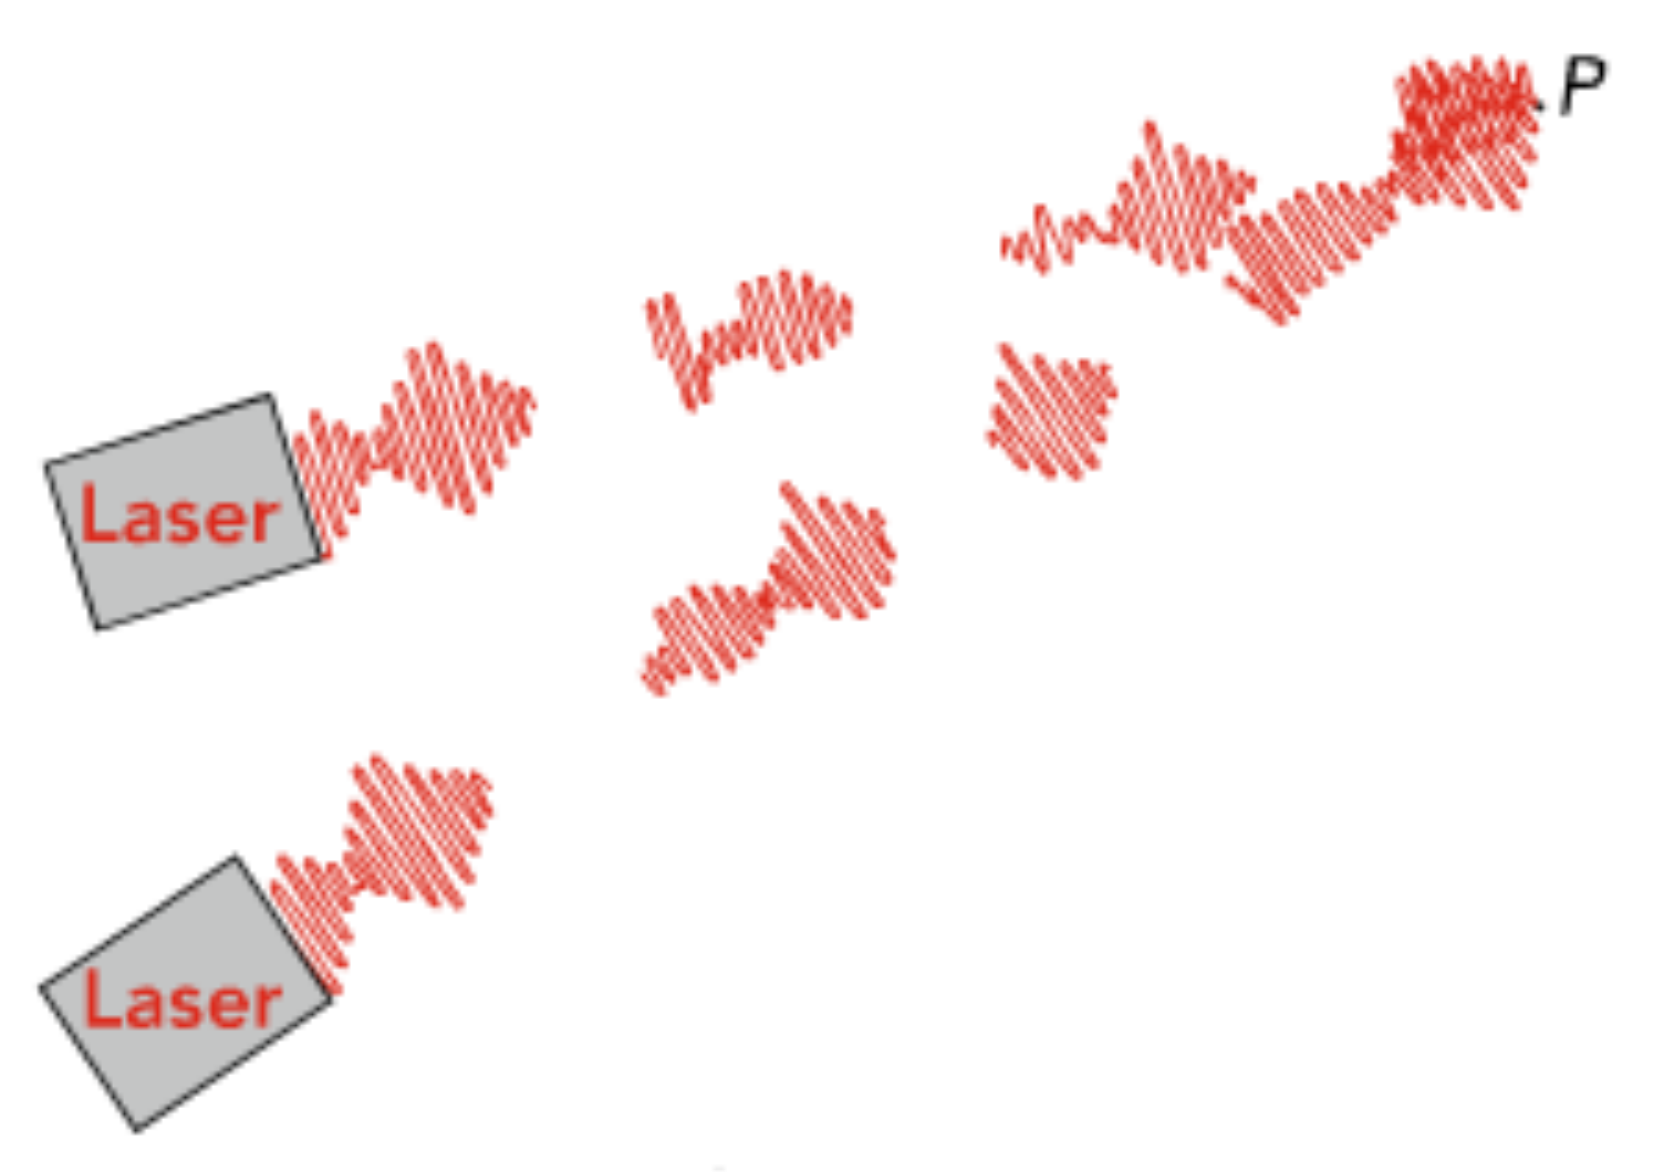
\includegraphics[width=\linewidth]{coherence}
	\end{center}
\end{minipage}
\hfill
\begin{minipage}{0.45\linewidth}
	\centering
	\captionsetup{justification=centering}
	\captionof{table}{Temps et longueurs de cohérence}
	\label{tab:tauclc}
	\begin{tabular}{lcc}
		\toprule
		Source               & $\tau_c$ (\si{s}) & $L_c$ (\si{m}) \\
		\midrule
		Lumière du Soleil    & \num{2e-15}       & \num{6e-7}     \\
		Ampoule              & \num{3e-14}       & \num{1e-5}     \\
		Raie rouge hydrogène & \num{1e-11}       & \num{4e-3}     \\
		Laser hélium-néon    & \num{1e-9}        & \num{3e-1}     \\
		\bottomrule
	\end{tabular}
\end{minipage}

\subsection{Intensité lumineuse}
La période (temporelle) typique d'une onde lumineuse est de l'ordre de
\SI{e-15}{s}, ou $\approx \SI{1}{fs}$~: c'est une échelle de temps
infinitésimale bien inférieure au temps de détection de n'importe quel capteur
optique~: l'œil humain a un temps de réponse $\approx \SI{e-1}{s}$, un capteur
CCD $\approx \SI{e-6}{s}$. Ainsi, un récepteur optique n'est sensible
\textbf{qu'à l'énergie moyenne du signal}. Cette énergie est proportionnelle au
carré de la grandeur $s(\Mr,t)$ propagée par l'onde (ici électromagnétique), et
on définit donc
\begin{tcb}(defi){Définition}
	\textbf{L'intensité d'un signal} est reliée à l'amplitude de l'onde
	\textit{via} la relation
	\[\psw{\boxed{I = K \moy{s^2(\Mr,t)}}}\]
	avec $K$ une constante et $\moy{\cdot}$ la moyenne temporelle.
\end{tcb}
Ainsi, pour une onde monochromatique $s(\Mr,t) = A\cos(\wt+\f(\Mr))$, on aura
\[I = KA^2\moy{\cos^2(\wt+\f(\Mr))} = \frac{1}{2}KA^2\]
\begin{tcb}(ror){}
	\psw{
		L'intensité lumineuse d'une onde monochromatique est
		proportionnelle au carré de son amplitude.}
	\vspace{-10pt}
\end{tcb}

\subsection{Formule de \textsc{Fresnel}}
Soient 2 ondes lumineuses cohérentes et de même pulsation, d'amplitudes $A_1$ et
$A_2$, interférant en un point M. On a vu que le signal somme $s(t) = s_1(t) +
	s_2(t)$ avait une amplitude
\[A = \sqrt{A_1{}^2 + A_2{}^2 + 2A_1A_2\cos\D\f_{1/2}(\Mr)}\]
On trouve donc l'intensité $I(\Mr)$ en en prenant le carré et en multipliant par
$\frac{1}{2}K$~:
\begin{gather*}
	I(\Mr)
	= \frac{1}{2}KA^2
	= \frac{1}{2}KA_1{}^2 + \frac{1}{2}KA_2{}^2 +
	2\frac{1}{2}KA_1A_2\cos\D\f_{1/2}(\Mr)\\
	\text{avec}\quad
	I_1 = \frac{1}{2}KA_1{}^2
	\qet
	I_2 = \frac{1}{2}KA_2{}^2
	\qMath{on trouve}
	\sqrt{I_1I_2} = \frac{1}{2}KA_1A_2
\end{gather*}
Ainsi, on a~:
\begin{tcb}(prop){Formule de \textsc{Fresnel}}
	L'intensité lumineuse $I(\Mr)$ résultant de l'interférence de 2 ondes
	monochromatiques en un point M de l'espace s'écrit\footnote{cette formule
		sera fournie dans les énoncés}~:
	\[\psw{\boxed{I(\Mr) = I_1 + I_2 + 2\sqrt{I_1I_2}\cos\D\f_{1/2}(\Mr)}}\]
	Si $A_1 = A_2 = A_0$, c'est-à-dire $I_1 = I_2 = I_0$, alors
	\[\psw{\boxed{I(\Mr) = 2I_0(1+\cos\D\f_{1/2}(\Mr))}}\]
	Ainsi, selon la valeur de $\D\f_{1/2}(\Mr)$ ($2p\pi$ ou $(2p+1)\pi$), on trouve
	$I(\Mr) = \psw{4I_0}$ ou $I(\Mr) = \psw{0}$.
\end{tcb}

\vspace{-10pt}
\subsection{Chemin optique et déphasage}
La propagation des ondes lumineuses se fait dans des milieux avec des indices
optiques $n$ qui peuvent être différents, et donc avec des vitesses $v = c/n$
différentes. Pour continuer à travailler comme on le fait, il faut cependant que
la vitesse des signaux soient les mêmes (même fréquence et même longueur d'onde).
On définit ainsi le \textbf{chemin optique}~:
\begin{tcb}(defi){Chemin optique}
	Le trajet d'un rayon lumineux dans un milieu d'indice $n$ entre les points A
	et B s'écrit $(\ABr)$, et on a
	\psw{
		\[
			(\ABr) = n \cdot \ABr
		\]
	}
	\vspace{-15pt}
\end{tcb}

\begin{tcb}(demo)<lft>'l'{Démonstration}
	\psw{
		En effet, si l'onde 1 parcourt la distance $\ABr$ dans le milieu $n$,
		elle le fait à la vitesse $v = c/n$. Pour considérer qu'elle va à la
		vitesse $c = nv$, il faut multiplier la distance par $n$~:
		\begin{gather*}
			n\ABr = nvt
			\Lra
			n\ABr = ct
		\end{gather*}
		Tout se passe comme si \textbf{l'onde allait à la vitesse $c$ mais
			parcourait une distance $n$ fois plus grande}.}
\end{tcb}

Ainsi, pour les interférences optiques, le déphasage prend en
compte le ou les indice(s) rencontré(s)~:

\begin{tcb}(prop){Déphasage et différence de chemin optique}
	Le déphasage entre 2 ondes \textit{lumineuses} sur superposant en M est
	\[\psw{\boxed{\D\f_{1/2}(\Mr) = -k_0\de_{1/2}(\Mr) + \D\f_0}}\]
	\begin{itemize}
		\item $\de_{1/2}(\Mr) = (\SaMr) - (\SbMr)$ est la \textbf{différence de
			      chemin optique} au point M.
		\item $k_0 = \dfrac{2\pi}{\lambda_0}$ est le \textbf{vecteur d'onde dans
			      le vide} correspondant à la \textbf{longueur d'onde dans le vide}
		      des ondes.
		\item $\D\f_0 = \f_{01}-\f_{02}$ est la \textbf{différence de phase à
			      l'origine entre les sources}.
	\end{itemize}
\end{tcb}

\section{Expérience des trous d'\textsc{Young}}
\subsection{Introduction}

La nature de la lumière a été sujet à de grands débats durant de nombreux
siècles, entre vision corpusculaire et ondulatoire. C'est en 1802 que
l'expérience dite des «~trous d'\textsc{Young}~» a permis de confirmer la nature
ondulatoire de la lumière en réalisant une figure d'interférences
lumineuses.
\bigbreak
En effet, pour obtenir 2 sources lumineuses cohérentes il faut créer deux
sources secondaires provenant d'une \textbf{source unique} et qui ait un temps
de cohérence suffisamment grand. Une version moderne de cette expérience
consiste à pointer un unique laser de longueur d'onde $\lambda$ sur deux fentes
fines horizontales et parallèles~: ces fentes diffractent la lumière est se
comportent \textbf{comme deux sources cohérentes}.
\bigbreak
\noindent
\begin{minipage}{0.45\linewidth}
	La zone de l'espace où les faisceaux se superposent est appelé \textbf{champ
		d'interférences}. Sur un écran, on observe alors la figure ci-contre, avec
	des variations d'intensité lumineuse~:
	\begin{itemize}
		\item au milieu des zones claires (\textbf{maximum} local d'intensité)
		      on a des \textbf{interférences constructives}~;
		\item au milieu des zones sombres (\textbf{minimum} local d'intensité)
		      on a des \textbf{interférences destructives}.
	\end{itemize}
\end{minipage}
\hfill
\begin{minipage}{0.50\linewidth}
	\begin{center}
		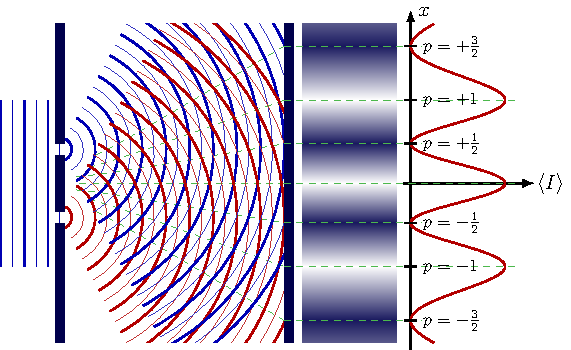
\includegraphics[width=\linewidth]{young_result}
	\end{center}
\end{minipage}

\bigbreak
\begin{tcb}(ror){}
	On appelle \textbf{interfrange} et on le note $i$ la \textit{distance}
	séparant deux milieux de franges brillantes (ou sombres) consécutives.
\end{tcb}

\subsection{Présentation}

Soit S une source lumineuse ponctuelle, monochromatique de longueur d'onde
$\lambda$, éclairant deux fentes fines horizontales et parallèles F$_1$ et F$_2$
distantes de $2a$, avec O au milieu. S est situé sur un axe optique
perpendiculaire à un écran placé à une distance $D$ très supérieure à $a$ (pour
l'approximation en ondes planes). Le milieu de propagation est l'air, d'indice
optique $n=1$.

\begin{figure}[htbp!]
	\centering
	\sswitch{
		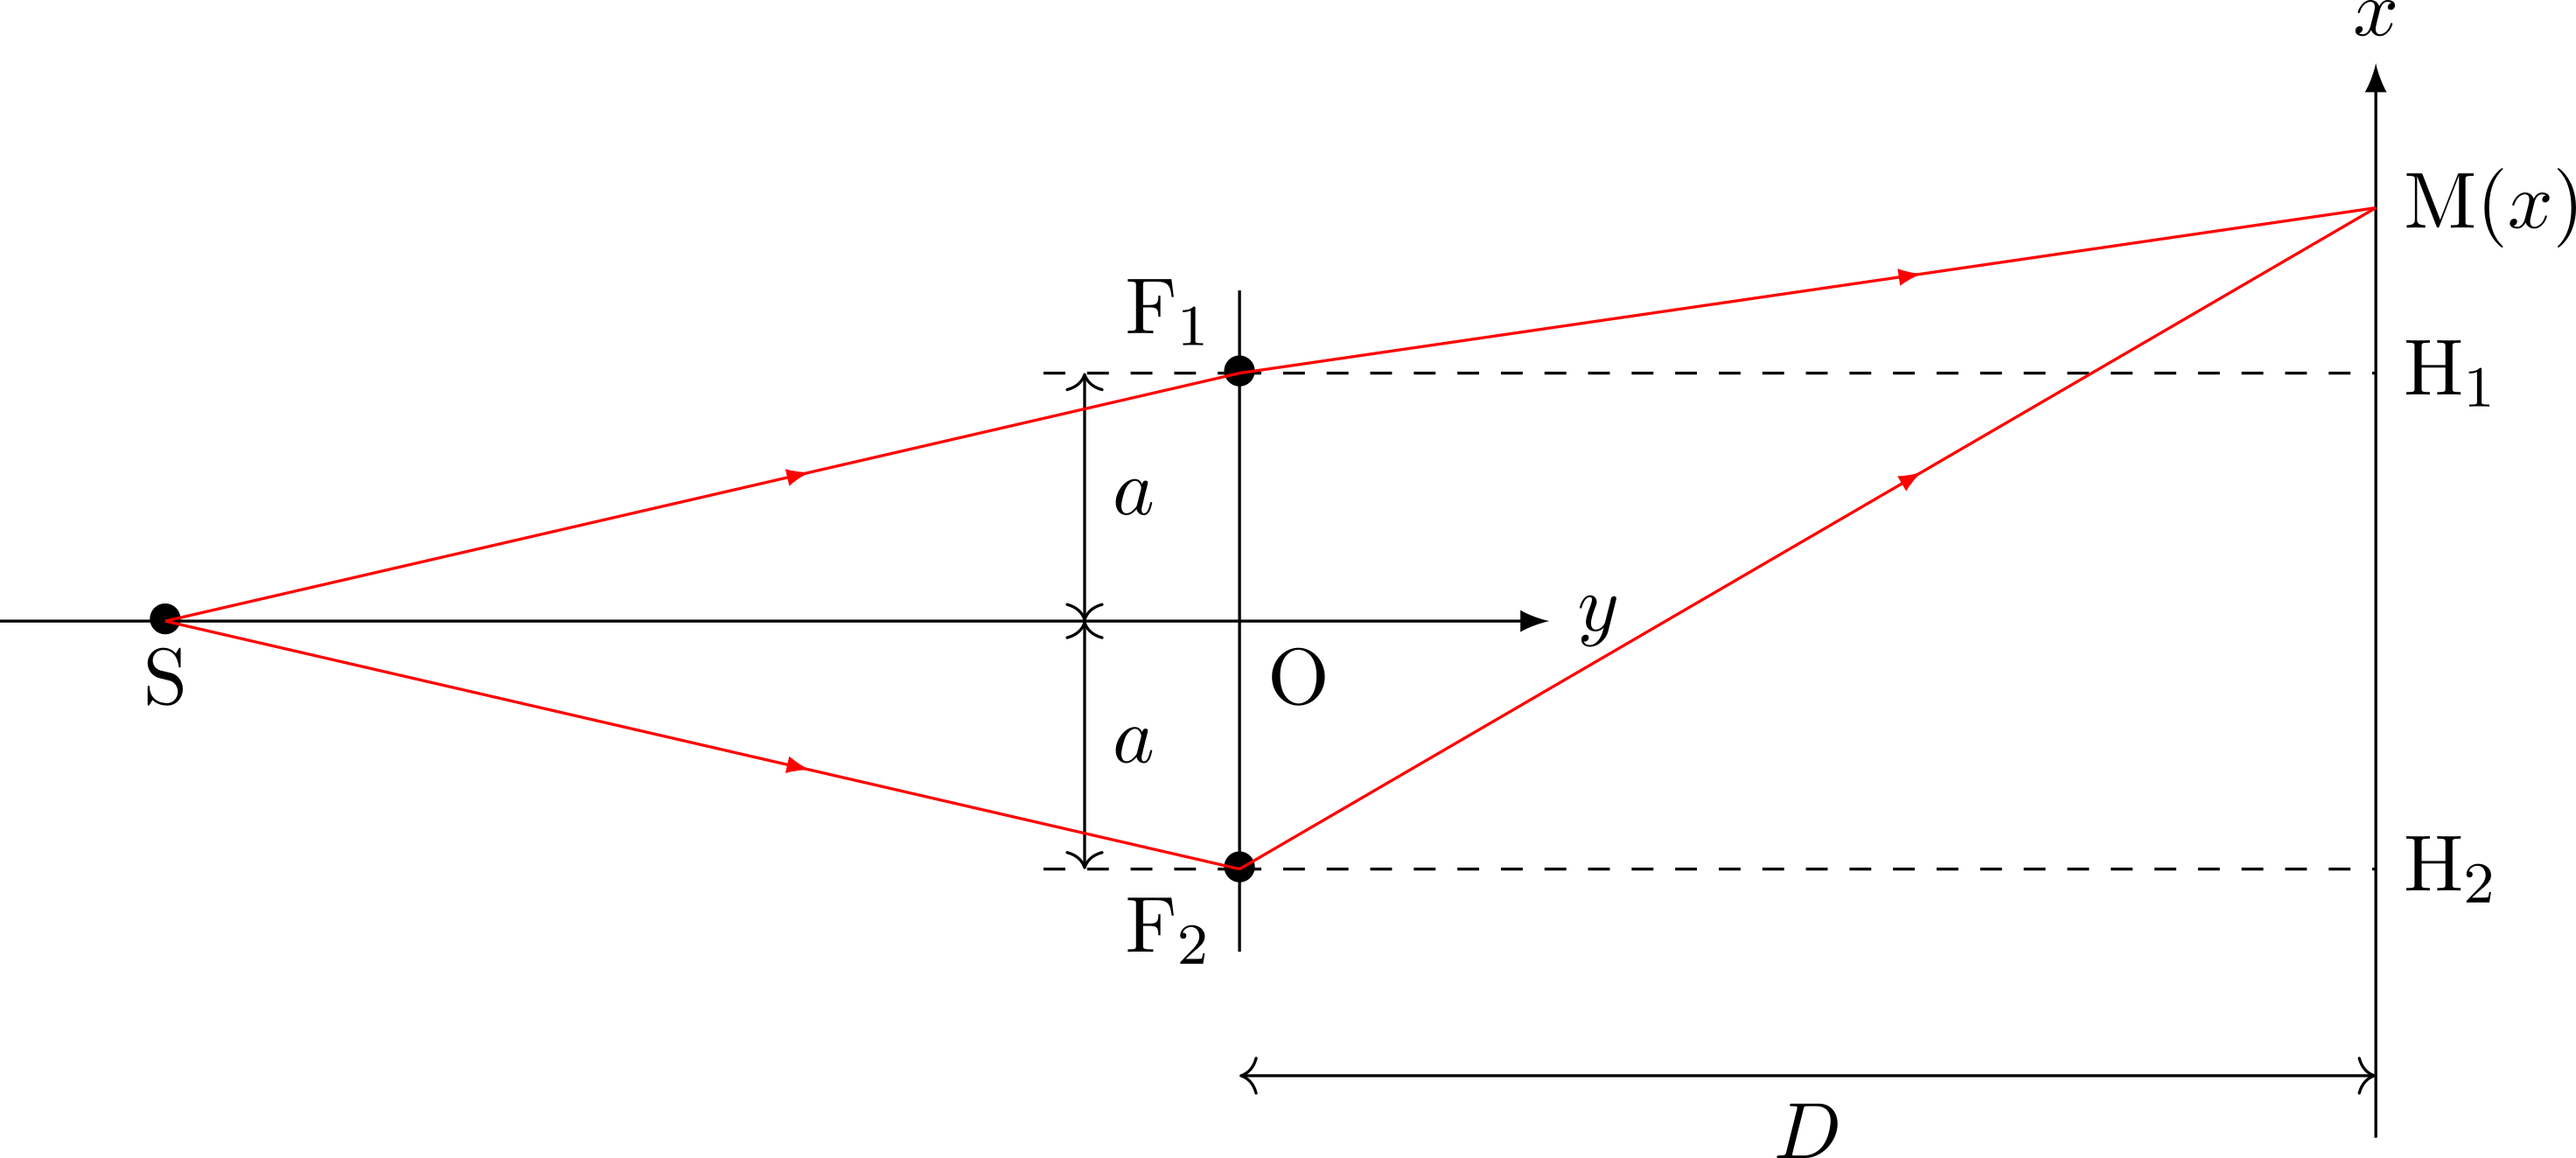
\includegraphics[width=.8\linewidth, draft=true]{yhole}
	}{
		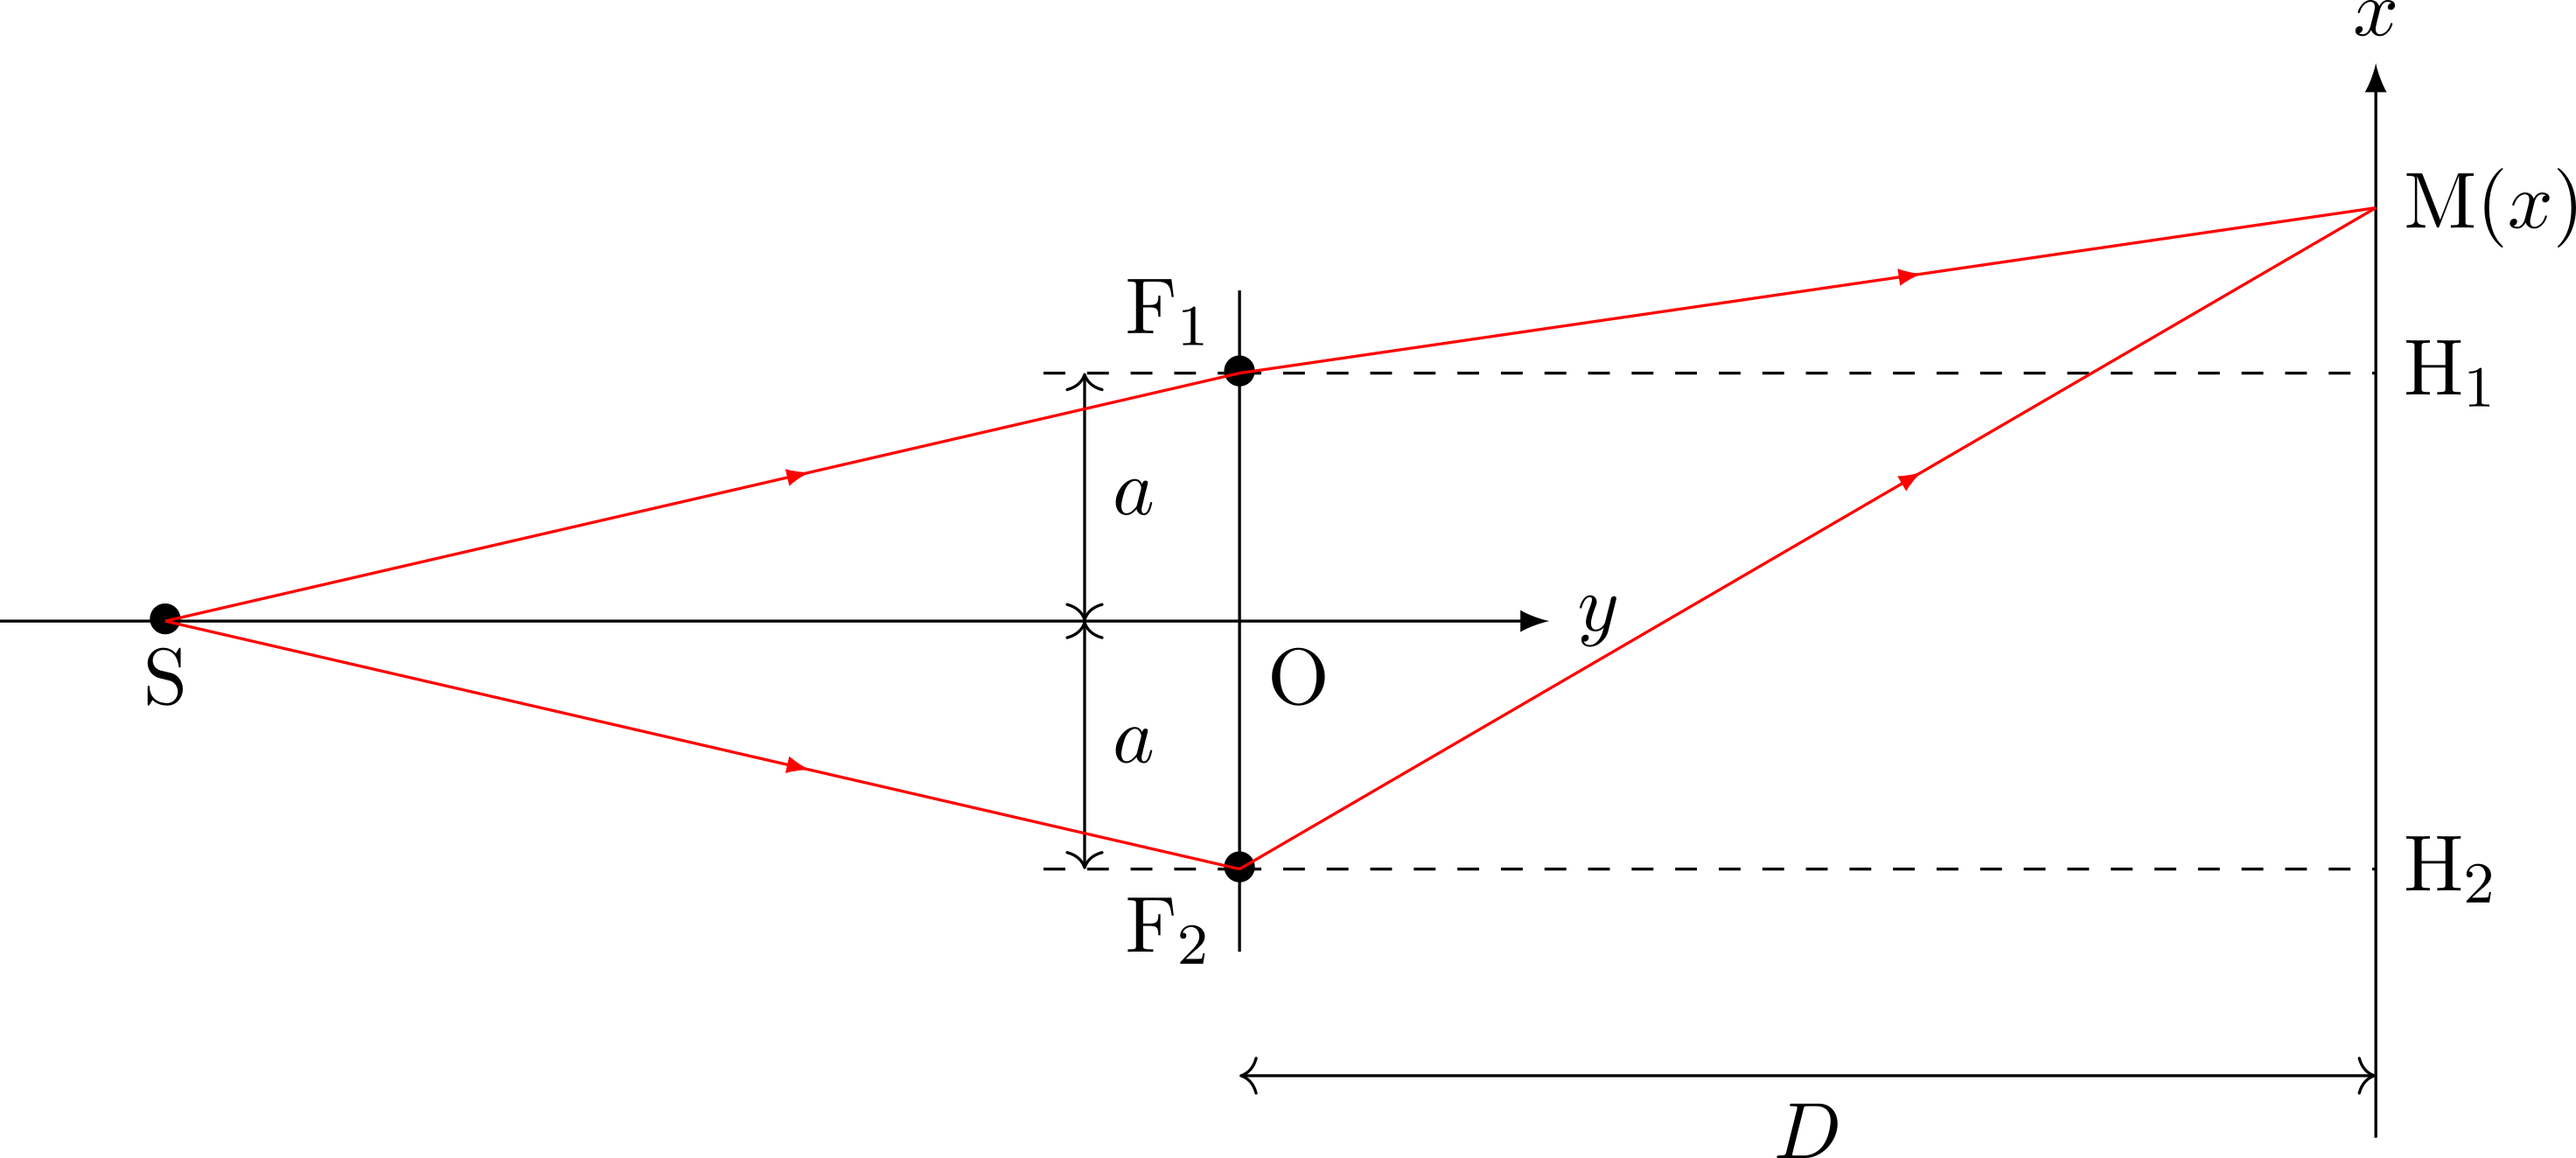
\includegraphics[width=.8\linewidth]{yhole}
	}
	\caption{Schéma des trous d'\textsc{Young}}
	\label{fig:yhole}
\end{figure}

On se limite au tracé de 2 rayons qui interfèrent au point M$(x)$, passant
chacun par une des fentes (voir Figure~\ref{fig:yhole}). On a alors
successivement~:

\begin{itemize}
	\item \textbf{Diffraction}~: les ondes passant par une fente sont en général
	      simplement coupées, mais quand l'ouverture est de l'ordre de la longueur
	      d'onde, on observe que le faisceau s'étale avec un motif
	      caractéristique. Plus l'ouverture est étroite, plus la taille du motif
	      est grande. Dans cette expérience, chaque trou créé une tâche de
	      diffraction, et ces deux tâches se superposent sur l'écran en créant des
	      interférences observables.
	\item \textbf{Interférence}~: avec la formule de \textsc{Fresnel}
	      \[I(\Mr) = I_1 + I_2 + 2\sqrt{I_1I_2}\cos\D\f_{1/2}(\Mr)\]
	      \begin{itemize}
		      \item Lorsque le déphasage est un multiple pair de $\pi$, soit
		            $\boxed{\D\f_{1/2} = 2p\pi}$, les interférences sont constructives.
		      \item Lorsque le déphasage est un multiple impair de $\pi$, soit
		            $\boxed{\D\f_{1/2} = (2p+1)\pi}$, les interférences sont
		            destructives.
	      \end{itemize}
\end{itemize}

On va donc déterminer le déphasage puis la différence de chemin de ces rayons,
pour finalement déterminer l'interfrange $i$.

\subsection{Détermination de l'interfrange}
\subsubsection{Calcul du déphasage}

Les phases des ondes 1 et 2 dues à leur propagation sont
\[\psw{
		\f_1({\Mr}) = -k_0({\rm SF_1 + F_1M})
		\qet
		\f_2({\Mr}) = -k_0({\rm SF_2 + F_2M})
	}\]
Or, SF$_1$ = SF$_2$, donc
\psw{
	\begin{gather*}
		\D\f_{1/2}(\Mr) = \f_1(\Mr) - \f_2(\Mr) = k_0(\rm F_2M - F_1M)\\
		\Leftrightarrow
		\boxed{\D\f_{1/2}(\Mr) = k_0\de_{2/1}(\Mr)}
	\end{gather*}}\vspace{-20pt}

\subsubsection{Calcul de la différence de chemin optique}
On cherche à exprimer $\rm F_1M$ et $\rm F_2M$ en fonction des grandeurs du
problème. Pour cela, on place les points H$_1$ et H$_2$ projetés orthogonaux de
F$_1$ et F$_2$ sur l'écran, créant ainsi deux triangles rectangles~: $\rm
	F_1H_1M$ et $\rm F_2H_2M$. Ainsi,
\psw{
	\begin{align*}
		{\rm
		F_1M^2 = F_1H_1{}^2 + H_1M^2}
		 & \qet
		{\rm
		F_2M^2 = F_2H_2{}^2 + H_2M^2} \\
		\Rightarrow
		{\rm F_1M} = \sqrt{D^2 + (x-a)^2}
		 & \qet
		{\rm F_2M} = \sqrt{D^2 + (x+a)^2}
	\end{align*}}
Avec $x\pm a \ll D$, on peut utiliser le développement limité
\[\sqrt{1+\ep} = 1 + \ep/2 + o(\ep)\]
Ainsi
\vspace*{-24pt}
\psw{
	\begin{align*}
		{\rm F_1M}               & = D\sqrt{1 + \left(\frac{x-a}{D}\right)^2} \\
		                         & \approx D \left( 1 + \frac{1}{2}
		\left(\frac{x-a}{D}\right)^2\right)                                   \\
		                         & = D + \frac{(x-a)^2}{2D}                   \\
		\text{et}\quad{\rm F_2M} & = D + \frac{(x+a)^2}{2D}
	\end{align*}}\vspace{-10pt}
D'où
\vspace*{-20pt}
\psw{\begin{align*}
		{\rm F_2M - F_1M}      & = \frac{(x+a)^2 - (x-a)^2}{2D}      \\
		\Leftrightarrow
		\de_{2/1}(\Mr)         & = \frac{(x+\cancel{a}+x-\cancel{a})
		\times(\bcancel{x}+a-(\bcancel{x}-a))}{2D}                   \\
		\Leftrightarrow
		\de_{2/1}(\Mr)         & = \frac{4ax}{2D}                    \\
		\Leftrightarrow
		\Aboxed{\de_{2/1}(\Mr) & = \frac{2ax}{D}}
	\end{align*}}\vspace{-10pt}

\subsubsection{Intensité lumineuse et interfrange}

Avec la formule de \textsc{Fresnel} avec $I_1 = I_2 = I_0$, on a
\[\psw{
		\boxed{I(\Mr) = 2I_0 \left( 1 + \cos\frac{4\pi ax}{\lambda D} \right)}
	}\]
Et ainsi, l'intensité est une fonction périodique selon $x$.

\begin{center}
	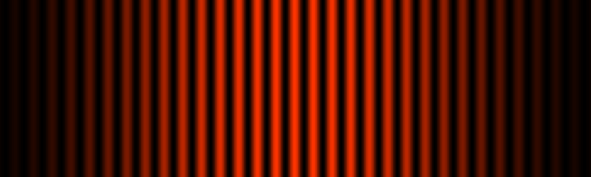
\includegraphics[scale=1]{young_intensity}
\end{center}

\begin{itemize}
	\item \textbf{Interférences constructives}~: les endroits où l'intensité est
	      maximale sont tels que
	      \psw{
		      \begin{gather*}
			      \D\f_{1/2}(\Mr) = 2p\pi
			      \quad\Longleftrightarrow\quad
			      \frac{2\pi\de(\Mr)}{\lambda} = 2p\pi
			      \quad\Longleftrightarrow\quad
			      \de(\Mr) = p\lambda\\
			      \Leftrightarrow
			      \boxed{x_p = p \frac{\lambda D}{2a}}
		      \end{gather*}}
	      \vspace{-10pt}
	\item \textbf{Interférences destructives}~: les endroits où l'intensité est
	      minimale sont tels que
	      \psw{
		      \begin{gather*}
			      \D\f_{1/2}(\Mr) = (2p+1)\pi
			      \quad\Longleftrightarrow\quad
			      \frac{2\pi\de(\Mr)}{\lambda} = (2p+1)\pi
			      \quad\Longleftrightarrow\quad
			      \de(\Mr) = \left(p+ \frac{1}{2}\right)\lambda\\
			      \Leftrightarrow
			      \boxed{x'_p = \left(p+ \frac{1}{2}\right) \frac{\lambda D}{2a}}
		      \end{gather*}}
	      \vspace{-10pt}
\end{itemize}

Ainsi, deux extrema d'intensité sont séparés de
\[\psw{
		i = x_{p+1} - x_p \Leftrightarrow \boxed{i = \frac{\lambda D}{2a}}
	}\]

Avec deux fentes séparées de \SI{0.20}{mm}, $\lambda = \SI{632}{nm}$ et $D =
	\SI{1.0}{m}$, on trouve
\[\boxed{i = \SI{1.6}{mm}}\]

Une autre animation est disponible en
ligne\footnote{\url{https://phyanim.sciences.univ-nantes.fr/Ondes/lumiere/interference_lumiere.php}}.

\end{document}
